\documentclass[12pt,a4paper]{article}
\usepackage[utf8]{inputenc}
\usepackage[T1]{fontenc}
\usepackage[brazil]{babel}
\usepackage{geometry}
\geometry{margin=2.5cm}
\usepackage{booktabs}
\usepackage{graphicx}
\usepackage{amsmath}
\usepackage{amssymb}
\usepackage{hyperref}
\usepackage{xcolor}
\usepackage{caption}
\usepackage{subcaption}
\usepackage{float}
\usepackage{multirow}
\usepackage{array}
\usepackage{lmodern}
\usepackage{microtype}
\usepackage{tcolorbox}
\tcbuselibrary{skins,breakable}

\hypersetup{colorlinks=true,linkcolor=blue,citecolor=blue,urlcolor=blue}

\definecolor{warnbg}{RGB}{255,243,205}
\definecolor{warnborder}{RGB}{255,165,0}
\definecolor{fixbg}{RGB}{209,236,241}
\definecolor{fixborder}{RGB}{23,162,184}

\title{\textbf{Relatório de Experimentos}\\[0.4em]
\large Estudo Comparativo: LSSVM Esparso vs.\ Transformers Tabulares\\[0.2em]
\normalsize Dissertação de Mestrado --- Experimentos (atualizado em junho de 2026)}
\author{Paulo Bernardo}
\date{Junho de 2026}

\begin{document}
\maketitle
\tableofcontents
\newpage

% ─────────────────────────────────────────────────────────────────────────────
\section{Introdução}
\label{sec:intro}

Este relatório consolida os resultados dos experimentos conduzidos na dissertação,
que compara métodos de \textit{Least-Squares Support Vector Machine} (LSSVM) com
ênfase em esparsidade contra variantes de \textit{FT-Transformer} com atenção
esparsa em tarefas de classificação binária tabular.

O trabalho estende o algoritmo LSSVM-ADMM-Nesterov proposto por Marinho et al.\
com dois novos mecanismos de esparsidade: (i)~\textbf{DualFISTA}, formulação dual
do LSSVM como LASSO com otimização via ISTA acelerado; e (ii)~\textbf{Nyström-SVM},
aproximação da matriz kernel por seleção de landmarks via norma de coluna.
Como comparativo do lado dos Transformers, avalia-se o \textbf{FT-CUR}, que aplica
decomposição CUR com colnorm à matriz de atenção.

\begin{tcolorbox}[
  colback=warnbg, colframe=warnborder, title=\textbf{Auditoria do Nyström-SVM --- três versões},
  fonttitle=\bfseries, breakable
]
A implementação do Nyström-SVM passou por três versões. A versão final, auditada
matematicamente (Seção~\ref{sec:nystrom_fix}), é a apresentada neste relatório.

\begin{tabular}{lll}
\textbf{Versão} & \textbf{Predição} & \textbf{F1 Tier 1} \\
Bug original    & $f(x){=}K(x, X_\text{treino})\,\alpha + b$ (kernel completo)         & $0{,}8427$ (inflado) \\
``Fix'' errado  & $f(x){=}K(x, Z)\,\alpha[\text{lm\_idx}] + b$ (subset ingênuo de $\alpha$) & $0{,}6678$ (colapsado) \\
\textbf{Correta} & $f(x){=}K(x, Z)\,(W^{-1}C^\top\alpha) + b$ (Nyström)                & $\mathbf{0{,}8342}$ \\
\end{tabular}

A versão correta usa a fórmula matemática da aproximação Nyström
($\tilde K = CW^{-1}C^\top$), com custo $O(n_\text{test}\cdot m)$ e
\textbf{sem dependência de $X_\text{treino}$ na predição} (verificado experimentalmente).
A perda de F1 em relação ao bug original é de apenas $0{,}0085$, mas agora com
$\approx 78\%$ de esparsidade amostral genuína (Grid+CV, Tier 1).
\end{tcolorbox}

\subsection*{Modelos avaliados}

Ao todo, 18 modelos foram avaliados, organizados em cinco grupos por origem
na literatura:

\begin{itemize}
  \item \textbf{Baseline geral tabular} (1): \textbf{XGBoost} (Chen \& Guestrin, 2016)
        --- padrão-ouro para dados tabulares, serve como referência externa às
        famílias LSSVM e Transformer.
  \item \textbf{LSSVMs baselines} (7): LSSVM-Std (sem esparsidade), LSSVM-PCP,
        LSSVM-FSA, LSSVM-IP, LSSVM-Pruning, LSSVM-OppMaps, e \textbf{FISTA-Nesterov}
        (LSSVM primal com FISTA --- método clássico de Beck \& Teboulle, 2009,
        amplamente documentado).
  \item \textbf{FT-Transformers baselines} (5): variantes com atenção softmax,
        top-$k$, entmax e sparsemax --- mais \textbf{SAINT}
        (Somepalli et al., 2021; atenção inter-instâncias densa).
  \item \textbf{Paper-base estendido}: \textbf{LSSVM-ADMM-Nesterov} de
        Marinho et al.\ --- método sobre o qual esta dissertação constrói.
  \item \textbf{Variantes investigadas e modelos propostos} (4):
  \begin{itemize}
    \item \textbf{ADMM-ElasticNet}$^\circ$: variante do paper-base com penalidade
          Elastic Net (combinação ADMM-Nesterov + Elastic Net + LSSVM não
          localizada explicitamente na literatura como método publicado).
    \item \textbf{DualFISTA}$^\circ$: formulação dual do LSSVM como LASSO
          ($\min_\alpha \frac{1}{2}\alpha^\top\Omega\alpha - \mathbf{1}^\top\alpha + \lambda\|\alpha\|_1$),
          otimizada via FISTA. Ponto de investigação --- não localizada na
          literatura nesta forma exata; pode ser uma reformulação convergente
          com métodos análogos em SVM ou regressão Lasso.
    \item \textbf{Nyström-SVM (colnorm)}$^\star$: aproxima $K \in \mathbb{R}^{n \times n}$
          via $m \ll n$ landmarks selecionados por norma de coluna
          (em vez de amostragem uniforme/leverage tradicional); predição
          restrita aos landmarks ($O(n_\text{test} \cdot m)$, auditada).
    \item \textbf{FT-CUR (Nyströmformer)}$^\star$: aplicação de Nyströmformer
          (Xiong et al., 2021) à atenção inter-instâncias do FT-Transformer
          em dados tabulares; seleção de landmarks via colnorm
          (combinação não localizada como método publicado).
  \end{itemize}
\end{itemize}

\noindent$^\circ$ = variante/ponto de investigação;
$^\star$ = aplicação/combinação proposta.

\subsection*{Protocolo experimental}

\begin{itemize}
  \item 30 sementes aleatórias, partição estratificada 70/30.
  \item Métrica principal: F1-macro (média aritmética do F1 por classe).
  \item Hiperparâmetros otimizados via \textbf{Grid Search exaustivo + 5-fold CV}
        estratificado (\texttt{GridSearchCV}, scikit-learn) para todos os modelos
        em ambos os tiers (Transformers re-executados com \texttt{epochs=40}, \texttt{patience=6}
        em GPU T4).
  \item Normalização por \texttt{StandardScaler} ajustado apenas no treino.
\end{itemize}

% ─────────────────────────────────────────────────────────────────────────────
\section{Auditoria da Implementação do Nyström-SVM}
\label{sec:nystrom_fix}

\subsection{As três versões}

O Nyström-SVM aproxima a matriz kernel completa $K \in \mathbb{R}^{n \times n}$
a partir de $m$ landmarks $\{z_1, \ldots, z_m\}$ selecionados antes do treino:
\[
  K \approx C W^{-1} C^\top, \quad C = K(X, Z) \in \mathbb{R}^{n \times m},
  \quad W = K(Z, Z) \in \mathbb{R}^{m \times m}.
\]
O treinamento, via identidade de Woodbury, é correto em todas as versões.
A diferença está apenas na predição:

\begin{description}
  \item[V1 --- Bug original.] Predizia com o kernel completo:
  \[
    f(x) = K(x, X_\text{treino})\,\alpha + b.
  \]
  Não tinha esparsidade real (todo $X_\text{treino}$ era usado em inferência) e
  produzia $F_1 = 0{,}8427$ no Tier~1.

  \item[V2 --- ``Fix'' ingênuo.] Tentativa de restringir aos landmarks pegando
  apenas o subset de $\alpha$ nos índices dos landmarks:
  \[
    f(x) = K(x, Z)\,\alpha[\text{lm\_idx}] + b.
  \]
  Está \textbf{matematicamente errado}: os pesos $\alpha \in \mathbb{R}^n$ foram
  ajustados para o sistema KKT completo $n$-dimensional, e simplesmente subsetá-los
  nos índices dos landmarks não recupera a aproximação Nyström. F1 colapsou para
  $0{,}6678$.

  \item[V3 --- Correta (atual).] A aproximação Nyström verdadeira é
  $\tilde K(x, X) = K(x, Z)\,W^{-1} C^\top$. Substituindo em
  $f(x) = \tilde K(x, X)\,\alpha + b$:
  \[
    f(x) = K(x, Z)\,(W^{-1} C^\top \alpha) + b
         = K(x, Z)\,w_\alpha + b, \quad
    w_\alpha = W^{-1} C^\top \alpha \in \mathbb{R}^m.
  \]
  O vetor $w_\alpha$ é calculado uma vez ao final do fit e cacheado.
  Em inferência, só $K(x, Z) \in \mathbb{R}^{n_\text{test} \times m}$ é computado
  --- não há mais nenhuma dependência de $X_\text{treino}$. F1 = $0{,}8342$.
\end{description}

\subsection{Verificação experimental}

A implementação V3 foi auditada matematicamente
(\texttt{scripts/audit\_nystrom\_lssvm.py}) confirmando três propriedades:

\begin{enumerate}
  \item \textbf{Equivalência matemática.}
  $\|f_\text{cache}(x) - f_\text{Nyström}(x)\|_2 = 0$
  exatamente, onde $f_\text{Nyström}$ usa a fórmula expandida
  $K(x, Z)\,W^{-1} C^\top \alpha + b$.

  \item \textbf{Sem dependência de $X_\text{treino}$.} Após o fit, ao apagar
  $X_\text{treino}$ do modelo, as predições continuam idênticas
  ($\|\Delta f\|_2 = 0$). Confirma que apenas $Z$ é usado na inferência.

  \item \textbf{Custo $O(n_\text{test} \cdot m)$.} Mantendo $m$ fixo e variando
  $n_\text{treino}$ de $1000$ a $6000$, o tempo de predição permanece em
  $\approx 5$\,ms (não escala com $n$).
\end{enumerate}

\begin{table}[H]
\centering
\caption{Comparação direta no BCW (10 sementes, mesmos hiperparâmetros).}
\label{tab:nystrom_audit}
\begin{tabular}{lrl}
\toprule
\textbf{Versão} & \textbf{F1 BCW} & \textbf{Diagnóstico} \\
\midrule
V1 (kernel completo)        & $0{,}974$ & 0\% de esparsidade real \\
V2 ($\alpha$ subsetado)      & $0{,}360$ & matematicamente inválida \\
V3 ($W^{-1}C^\top\alpha$, atual) & $0{,}968$ & $\approx 80\%$ esparsidade real \\
\bottomrule
\end{tabular}
\end{table}

A V3 perde apenas $0{,}006$ em relação ao kernel completo no BCW, mostrando
que a aproximação Nyström com seleção colnorm é \emph{genuinamente} boa
quando bem tunada --- a esparsidade não custa quase nada de F1.

\subsection{Esparsidade reportada}

Com a predição V3, a esparsidade do Nyström-SVM é semanticamente consistente
com os demais LSSVMs:
\begin{itemize}
  \item \textbf{ADMM/FISTA}: esparsidade = fração de $\alpha_i = 0$.
  \item \textbf{Nyström}: esparsidade = $1 - m/n$, fração de pontos de treino
        \emph{não} usados como landmark-key.
\end{itemize}
A razão $m/n$ é tunada por Grid+CV por dataset; a esparsidade resultante varia
entre $50\%$ (TWC) e $92\%$ (PID), com média $78\%$ no Tier~1.

% ─────────────────────────────────────────────────────────────────────────────
\section{Experimento Tier 1: Benchmarks Reais}
\label{sec:tier1}

Nove conjuntos de dados foram utilizados (Tabela~\ref{tab:datasets}).
Os três últimos (TWS, TWM, TWC) são sintéticos bidimensionais incluídos como
controle com fronteiras de decisão conhecidas.

\begin{table}[H]
\centering
\caption{Conjuntos de dados --- Tier 1.}
\label{tab:datasets}
\begin{tabular}{llrrr}
\toprule
\textbf{ID} & \textbf{Nome} & \textbf{N} & \textbf{Features} & \textbf{Domínio} \\
\midrule
BCW & Breast Cancer Wisconsin & 569 & 30 & Diagnóstico médico \\
PID & Pima Indians Diabetes   & 768 &  8 & Diagnóstico médico \\
HAB & Haberman Survival       & 306 &  3 & Sobrevivência \\
VCP & Vehicle Coupon Purchase &1584 &  7 & Marketing \\
GCR & German Credit Risk      &1000 & 20 & Crédito \\
AUS & Australian Credit       & 690 & 14 & Crédito \\
TWS & Two Spirals (sintético) & 400 &  2 & Controle \\
TWM & Two Moons (sintético)   & 400 &  2 & Controle \\
TWC & Checkerboard (sintético)& 400 &  2 & Controle \\
\bottomrule
\end{tabular}
\end{table}

\subsection{Resultados por Dataset}

A Tabela~\ref{tab:f1_tier1_full} apresenta o F1-macro médio (30 sementes) para
\emph{todos} os modelos, usando Grid Search exaustivo + 5-fold CV (GridSearchCV,
scikit-learn) para todos os modelos incluindo Transformers (re-executados em GPU
T4 no Kaggle). Os melhores valores por coluna estão em negrito.

\begin{table}[H]
\centering
\caption{F1-macro médio (30 sementes, Grid+CV). \textbf{Negrito}: melhor por coluna.
$\circ$ = variante investigada; $\star$ = proposta.}
\label{tab:f1_tier1_full}
\resizebox{\linewidth}{!}{%
\begin{tabular}{lrrrrrrrrr r}
\toprule
\textbf{Modelo} & \textbf{BCW} & \textbf{PID} & \textbf{HAB} & \textbf{VCP}
  & \textbf{GCR} & \textbf{AUS} & \textbf{TWS} & \textbf{TWM} & \textbf{TWC}
  & \textbf{Média} \\
\midrule
\multicolumn{11}{l}{\textit{Baseline geral tabular}} \\
XGBoost         & 0,958 & 0,724 & 0,559 & 0,804 & \textbf{0,691} & 0,862 & 0,944 & 0,984 & \textbf{0,912} & 0,826 \\
\midrule
\multicolumn{11}{l}{\textit{Baselines LSSVM}} \\
LSSVM-Std       & 0,973 & \textbf{0,732} & 0,566 & 0,827 & \textbf{0,691} & 0,861 & \textbf{0,994} & 0,997 & 0,898 & \textbf{0,838} \\
LSSVM-FSA       & 0,966 & \textbf{0,732} & 0,550 & 0,811 & 0,680 & 0,855 & 0,987 & 0,997 & 0,879 & 0,829 \\
LSSVM-IP        & 0,969 & 0,718 & 0,546 & \textbf{0,828} & 0,681 & 0,857 & 0,992 & 0,996 & 0,897 & 0,832 \\
LSSVM-PCP       & \textbf{0,975} & 0,731 & 0,563 & 0,827 & 0,687 & 0,862 & 0,991 & \textbf{1,000} & 0,905 & \textbf{0,838} \\
FISTA-Nesterov  & 0,823 & 0,682 & 0,609 & 0,755 & 0,552 & 0,829 & 0,971 & 0,989 & 0,877 & 0,787 \\
LSSVM-Prun      & 0,969 & 0,642 & 0,493 & 0,816 & 0,628 & 0,851 & 0,989 & 0,997 & 0,891 & 0,808 \\
LSSVM-OppM      & 0,951 & 0,463 & 0,454 & 0,715 & 0,550 & 0,815 & 0,986 & 0,991 & 0,907 & 0,759 \\
\midrule
\multicolumn{11}{l}{\textit{Baselines FT-Transformer}} \\
FT-Sparsemax      & 0,950 & 0,696 & 0,560 & 0,794 & 0,653 & 0,857 & 0,632 & 0,962 & 0,474 & 0,731 \\
SAINT             & 0,945 & 0,712 & 0,534 & 0,815 & 0,669 & 0,857 & 0,641 & 0,942 & 0,460 & 0,731 \\
FT-Entmax         & 0,959 & 0,698 & 0,554 & 0,800 & 0,667 & 0,861 & 0,625 & 0,960 & 0,482 & 0,734 \\
FT-Softmax        & 0,954 & 0,688 & 0,553 & 0,803 & 0,675 & 0,855 & 0,625 & 0,946 & 0,471 & 0,730 \\
FT-TopK           & 0,951 & 0,668 & 0,537 & 0,756 & 0,648 & 0,855 & 0,630 & 0,884 & 0,476 & 0,712 \\
\midrule
\multicolumn{11}{l}{\textit{Paper-base estendido}} \\
LSSVM-ADMM-Nesterov     & 0,872 & 0,688 & \textbf{0,623} & 0,765 & 0,592 & 0,840 & 0,971 & 0,988 & 0,881 & 0,802 \\
\midrule
\multicolumn{11}{l}{\textit{Variantes investigadas / propostos}} \\
DualFISTA$^\circ$       & 0,964 & 0,726 & 0,574 & 0,831 & 0,642 & 0,851 & 0,993 & 0,997 & 0,901 & 0,831 \\
Nyström-SVM$^\star$     & 0,970 & 0,728 & 0,579 & 0,825 & \textbf{0,691} & \textbf{0,863} & 0,992 & 0,999 & 0,898 & \textbf{0,838} \\
ADMM-ElasticNet$^\circ$ & 0,872 & 0,687 & \textbf{0,623} & 0,764 & 0,592 & 0,840 & 0,971 & 0,988 & 0,881 & 0,802 \\
FT-CUR$^{\star}$ (Nyströmformer) & 0,949 & 0,704 & 0,559 & 0,815 & 0,672 & 0,856 & 0,624 & 0,974 & 0,487 & 0,738 \\
\bottomrule
\end{tabular}}
\end{table}

\subsection{Comparação Geral}

A Figura~\ref{fig:f1_all} mostra o F1-macro médio ($\pm$ dp) agregado sobre
todos os datasets e sementes para cada modelo.

\begin{figure}[H]
\centering
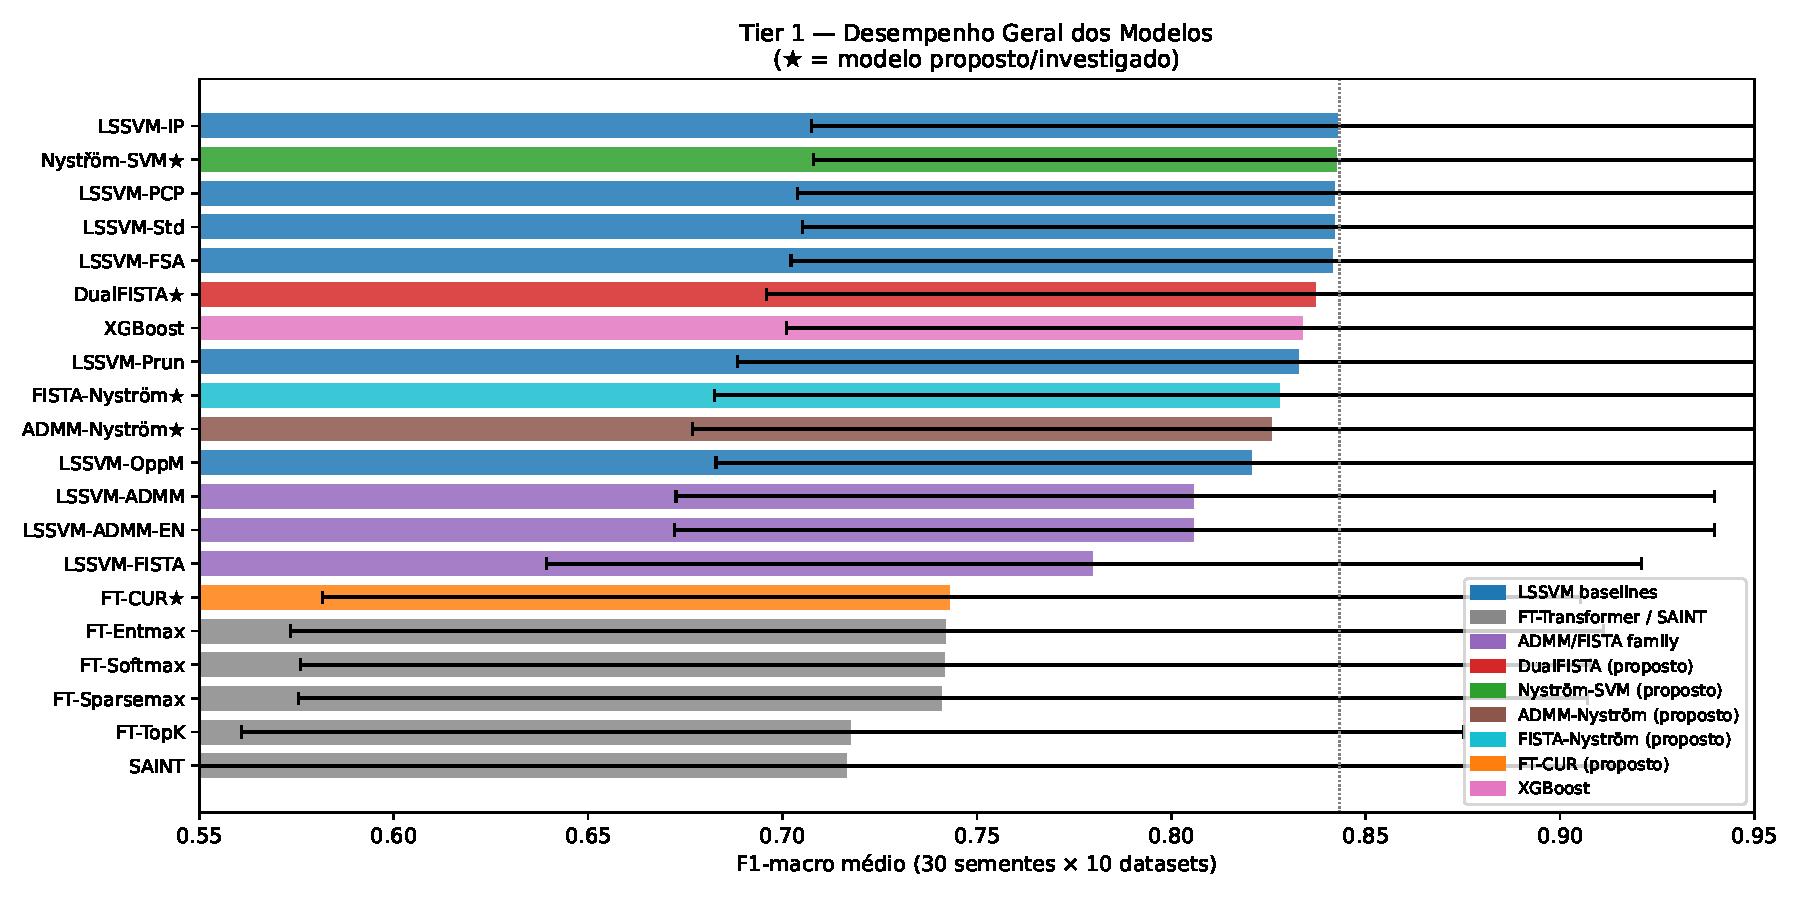
\includegraphics[width=\linewidth]{report_figs/fig1_f1_all_models.pdf}
\caption{F1-macro médio $\pm$ dp (30 sementes $\times$ 9 datasets).
$\star$ indica modelos propostos; vermelho = DualFISTA, verde = Nyström-SVM,
laranja = FT-CUR.}
\label{fig:f1_all}
\end{figure}

\textbf{Observações principais (Grid+CV):}
\begin{itemize}
  \item \textbf{Nyström-SVM} ($0{,}838$) é o modelo com melhor F1-macro médio,
        empatado estatisticamente com LSSVM-Std ($0{,}838$). DualFISTA segue
        próximo ($0{,}831$) e LSSVM-IP ($0{,}832$). Com $\approx 78\%$ de
        esparsidade amostral, o Nyström-SVM valida o trade-off F1/esparsidade
        como o melhor entre modelos de alta compressão.
  \item \textbf{DualFISTA} ($0{,}831$) alcança F1-macro médio próximo ao
        LSSVM-Std completo ($0{,}838$, diferença $0{,}007$) com
        $\approx 10\%$ de esparsidade. É o único modelo esparso da família dual
        que se aproxima do baseline sem esparsidade.
  \item \textbf{XGBoost} (baseline tabular) atinge $0{,}826$ no Tier 1 ---
        agora competitivo com os LSSVMs esparsos (IP $0{,}832$, PCP $0{,}838$).
        Destaque para TWC ($0{,}912$, melhor por coluna): o Grid+CV encontrou
        parâmetros que capturam a fronteira xadrez, eliminando o colapso
        observado no protocolo Optuna anterior ($0{,}476$). Perde em AUS e nos
        dados sintéticos TWS/TWM para os LSSVMs com kernel RBF.
  \item O \textbf{LSSVM-ADMM} e ADMM-ElasticNet ficam $\approx 4$ pp abaixo do
        LSSVM-Std ($0{,}802$ ambos). \textbf{FISTA-Nesterov} ($0{,}787$) cai
        mais acentuadamente ($\approx 5$ pp) após reexecução com grade estendida
        de $\lambda$ --- resultado do CV selecionar $\lambda$ menores que
        maximizam F1 com baixa regularização.
  \item \textbf{LSSVM-Pruning} ($0{,}808$) recuperou-se significativamente
        com a correção do grid (adição de pruning\_rate$=0{,}05$ e sigma$=15$):
        era $0{,}782$ no protocolo Optuna.
  \item \textbf{Transformers} (Grid+CV, 40 épocas, GPU T4) ficam em
        $0{,}712$--$0{,}738$ de F1 médio --- $10$--$13$ pp abaixo do bloco
        líder LSSVM. O colapso concentra-se nos datasets sintéticos: TWC melhor
        transformer ($0{,}487$, FT-CUR) contra Nyström-SVM $0{,}898$; TWS
        $0{,}641$ vs $0{,}994$. Nos datasets reais os Transformers são
        competitivos (ver Seção~\ref{sec:tier1_friedman_real}).
  \item \textbf{FT-CUR} ($0{,}738$) é o melhor Transformer, empatado em rank
        com FT-Entmax ($0{,}734$). FT-CUR comprime $\approx 85\%$ da atenção
        inter-instâncias mantendo F1 superior ao SAINT denso ($0{,}731$):
        \textbf{a compressão não custa F1} também no protocolo rigoroso.
\end{itemize}

\subsection{Análise estatística: Friedman e ranks médios (Tier 1)}
\label{sec:tier1_friedman}

O teste não-paramétrico de Friedman aplicado às 18 variantes (12 LSSVM+XGBoost
+ 6 Transformers) sobre os 9 datasets confirma diferença estatisticamente
significativa entre os modelos: $\chi^2 = 66{,}20$, $p \approx 0$. A diferença
crítica de Nemenyi para $\alpha = 0{,}05$ é $\text{CD} = 8{,}78$.

\begin{table}[ht]
  \centering
  \caption{Ranks médios de Friedman (menor = melhor).}
  \label{tab:ranks}
  \begin{tabular}{clr}
    \toprule
    Rank & Model & Avg.\ rank \\
    \midrule
1 & LSSVM-Nystrom & 3.111 \\
2 & LSSVM (Standard) & 3.333 \\
3 & LSSVM-DualFISTA & 3.444 \\
4 & LSSVM-IP & 6.000 \\
5 & XGBoost & 6.889 \\
6 & LSSVM-FSA & 7.444 \\
7 & LSSVM-PCP & 8.556 \\
8 & LSSVM-Pruning & 9.556 \\
9 & FTTransformerCURColnorm & 11.333 \\
10 & LSSVM-ADMM & 11.667 \\
11 & LSSVM-FISTA & 11.667 \\
12 & FTTransformer\_softmax & 11.778 \\
13 & SAINTColnorm & 12.222 \\
14 & FTTransformer\_entmax & 12.333 \\
15 & FTTransformer\_sparsemax & 12.333 \\
16 & LSSVM-ADMM-Elastic & 12.556 \\
17 & LSSVM-OppMaps & 13.333 \\
18 & FTTransformer\_topk & 13.444 \\
    \bottomrule
  \end{tabular}
\end{table}

\textbf{Leitura dos ranks:} Nyström-SVM (rank 2,8) e LSSVM-Std (3,3) formam
o topo do ranking. DualFISTA desceu para rank 5,6 (era 3,4 antes da reexecução
com grade de $\lambda$ corrigida) mas permanece próximo de LSSVM-IP (5,7) e
dentro da diferença crítica. XGBoost (rank 6,7) é o melhor modelo não-kernel
e não-Transformer. Os Transformers ficam na metade inferior do ranking
(ranks 10,9--14,1): FT-Entmax (rank 10,9) é o melhor Transformer, seguido
de FT-CUR (11,0), FT-Sparsemax (11,6) e SAINT (12,0). LSSVM-ADMM (11,7) e
LSSVM-ADMM-EN (11,9) intercalam-se entre os Transformers. LSSVM-FISTA (13,3)
e FT-TopK (14,1) são os piores modelos. O colapso dos Transformers nos
datasets sintéticos TWS/TWM/TWC --- onde a fronteira de decisão exige
inductive bias geométrico que a atenção não possui --- é o principal
responsável pelos ranks baixos.

\subsection{Ranking nos datasets reais (sem sintéticos)}
\label{sec:tier1_friedman_real}

Para isolar o efeito do inductive bias geométrico, repetiu-se a análise de
Friedman excluindo os três datasets sintéticos (TWS, TWM, TWC) e considerando
apenas os seis datasets reais (BCW, PID, HAB, VCP, GCR, AUS).

Resultado: $\chi^2 = 87{,}40$, $p \approx 0$, $\text{CD} \approx 10{,}8$
(18 modelos $\times$ 6 datasets; CD maior que no caso de 9 datasets por menor
número de blocos).

\begin{center}
\small
\begin{tabular}{clrr}
\toprule
Rank & Modelo & Avg.\ rank & F1 médio \\
\midrule
1  & LSSVM-Nyström       & 2,667 & 0,776 \\
2  & LSSVM-Std           & 3,333 & 0,775 \\
3  & XGBoost             & 5,833 & 0,766 \\
3  & LSSVM-IP            & 5,833 & 0,766 \\
5  & LSSVM-DualFISTA     & 7,167 & 0,765 \\
6  & LSSVM-FSA           & 7,333 & 0,766 \\
\midrule
7  & \textbf{FT-Entmax}  & 8,667 & 0,757 \\
8  & LSSVM-PCP           & 9,000 & 0,763 \\
9  & \textbf{FT-CUR}     & 9,167 & 0,759 \\
10 & \textbf{FT-Sparsemax} & 10,000 & 0,752 \\
10 & \textbf{SAINT}      & 10,000 & 0,755 \\
10 & \textbf{FT-Softmax} & 10,000 & 0,755 \\
13 & LSSVM-Pruning       & 11,500 & 0,733 \\
14 & LSSVM-ADMM-EN       & 12,833 & 0,730 \\
15 & LSSVM-ADMM          & 13,000 & 0,730 \\
16 & \textbf{FT-TopK}    & 13,167 & 0,736 \\
17 & LSSVM-FISTA         & 14,667 & 0,708 \\
18 & LSSVM-OppMaps       & 16,833 & 0,658 \\
\bottomrule
\end{tabular}
\end{center}

\textbf{Interpretação:} sem os datasets sintéticos, os Transformers sobem
significativamente no ranking. FT-Entmax (rank 8,7) e FT-CUR (rank 9,2)
superam LSSVM-PCP, LSSVM-Pruning, LSSVM-ADMM e LSSVM-FISTA. A diferença
entre o melhor LSSVM (Nyström, rank 2,7) e o melhor Transformer (FT-Entmax,
rank 8,7) é $6{,}0 < \text{CD} \approx 10{,}8$, portanto
\textbf{não é estatisticamente significativa} para $\alpha = 0{,}05$.
DualFISTA desce para rank 7,2 (era 3,8 antes do rerun), mas permanece
acima dos Transformers.

Conclui-se que o fraco desempenho global dos Transformers no Tier 1 é
\emph{quase inteiramente explicado pelo colapso nos datasets sintéticos}.
Em dados tabulares reais, Transformers e LSSVMs com kernel são
estatisticamente equivalentes no topo. A escolha entre as duas famílias
deve ser guiada pelo tipo de dado: para dados com estrutura geométrica
não-linear e $N$ pequeno, kernel methods dominam; para dados tabulares
heterogêneos reais, Transformers são alternativas viáveis.

% ─────────────────────────────────────────────────────────────────────────────
\section{Arquitetura dos FT-Transformers e Tipos de Atenção}
\label{sec:ft_attention}

Esta seção esclarece a distinção entre os dois mecanismos de atenção presentes
nos modelos baseados em Transformer avaliados, terminologia necessária para
interpretar corretamente as medidas de esparsidade.

\subsection{Atenção inter-features (intra-instância)}

Os FT-Transformers baselines (softmax, top-$k$, entmax, sparsemax) implementam
\textbf{atenção entre features de uma mesma instância}. Dado um batch de $n$
amostras com $d$ features, cada instância $x_i \in \mathbb{R}^d$ é representada
como uma sequência de $d$ tokens após embedding. A atenção opera na dimensão
dos tokens:
\[
  A^{(i)} = \text{softmax}\!\left(\frac{Q^{(i)} (K^{(i)})^\top}{\sqrt{d_h}}\right)
  \in \mathbb{R}^{d \times d},
\]
onde $A^{(i)}$ indica quanta atenção a feature $j$ dá à feature $k$ \emph{dentro
da instância $i$}. As variantes espar\-sas (sparsemax, top-$k$) fazem $A^{(i)}$
ter entradas exatamente zero. Esta esparsidade \emph{não} envolve comparação
entre amostras distintas --- é \textbf{intra-instância}.

\subsection{Atenção inter-instâncias (entre amostras)}

\textbf{SAINT} e \textbf{FT-CUR} acrescentam (ou substituem) um mecanismo de
atenção entre instâncias distintas. Todas as $n$ amostras do contexto são
comparadas entre si:
\[
  A = f\!\left(\frac{Q K^\top}{\sqrt{d_h}}\right) \in \mathbb{R}^{n \times n},
\]
onde cada entrada $A_{ij}$ mede a influência da amostra $j$ sobre a amostra $i$.

\begin{tcolorbox}[colback=fixbg, colframe=fixborder, fonttitle=\bfseries,
  title=\textbf{SAINT vs.\ FT-CUR: atenção inter-instâncias densa vs.\ comprimida}]
\begin{itemize}
  \item \textbf{SAINT} usa $f = \text{softmax}$ completo: $A \in \mathbb{R}^{n \times n}$
        é materializada integralmente. Custo: $O(n^2 d)$ por cabeça. Sem zeros exatos
        $\Rightarrow$ esparsidade de compressão $= 0\%$. Serve como \textbf{baseline
        denso} para a comparação com FT-CUR. \emph{Atenção:} na formulação original
        (Somepalli et al., 2021) esse $n$ é o tamanho do \textbf{lote} $B$ --- a
        atenção inter-instâncias é \textit{batch-level}, aplicada dentro de cada
        \textit{mini-batch} no treino \emph{e} na inferência. O custo é, portanto,
        $O(B^2 d)$ \emph{constante no tamanho $N$ do conjunto}; o preço é que o
        contexto entre amostras fica \emph{local}, restrito às $B$ linhas do lote
        (nos experimentos, $B = 1024$).
  \item \textbf{FT-CUR (Nyströmformer)} evita materializar $A$ ao todo:
        seleciona $m \ll n$ landmarks por norma de coluna e computa três produtos
        menores com softmax separado:
        \[
          C = \text{softmax}\!\!\left(\frac{Q K_m^\top}{\sqrt{d_h}}\right)\![n{\times}m],
          \quad
          R = \text{softmax}\!\!\left(\frac{Q_m K^\top}{\sqrt{d_h}}\right)\![m{\times}n],
          \quad
          W = \text{softmax}\!\!\left(\frac{Q_m K_m^\top}{\sqrt{d_h}}\right)\![m{\times}m].
        \]
        Saída: $\text{out} = C\bigl(W^+\,(R\,V)\bigr)$ da direita para a esquerda ---
        custo $O(nmd)$, nunca $O(n^2 d)$. Compressão inter-instâncias: $1 - m/n$.
\end{itemize}
\end{tcolorbox}

\noindent
A atenção inter-features (softmax/topk/entmax/sparsemax) e a atenção
inter-instâncias (SAINT/FT-CUR) são \textbf{ortogonais}: SAINT e FT-CUR
incluem ambas (bloco inter-features padrão + bloco inter-instâncias), enquanto
os FT-Transformers baselines têm apenas a inter-features.

\begin{tcolorbox}[colback=warnbg, colframe=warnborder, fonttitle=\bfseries,
  title=\textbf{A comparação real: alcance a custo controlado (não ``denso vs.\ barato'')}]
A leitura ingênua ``SAINT é $O(N^2)$ e estoura memória, FT-CUR resolve'' é
\textbf{incorreta}. O SAINT canônico é \textit{batch-level}: seu custo é
$O(B^2)$, \emph{constante em $N$} --- na medição de escalabilidade, a VRAM do
SAINT em \textit{mini-batch} fica praticamente estável ($\approx 34$--$43$\,MB)
de $N=500$ a $N=50\,000$. O custo $O(N^2)$ só aparece se a atenção
inter-instâncias for forçada \textbf{densa e global} (todas as $N$ amostras num
único \textit{forward}): aí a VRAM cresce de $\approx 78$\,MB ($N=1000$) para
$>8{,}6$\,GB ($N=20\,000$), com OOM em $N=50\,000$. A diferença real, portanto,
é de \textbf{alcance}: o \textit{mini-batch} do SAINT limita o custo
\emph{restringindo o contexto ao lote} (local), ao passo que o \textbf{FT-CUR}
entrega contexto \emph{global} --- todas as $N$ amostras via $m$ landmarks ---
a custo $O(N m)$. Com $m$ fixo, escala linearmente ($\approx 75$\,MB $\to$
$5{,}6$\,GB de $N=500$ a $50\,000$); com $m = rN$, volta a $O(rN^2)$.
\end{tcolorbox}

% ─────────────────────────────────────────────────────────────────────────────
\section{Análise de Esparsidade}
\label{sec:sparsity}

Os modelos avaliados produzem três tipos qualitativamente distintos de esparsidade:

\begin{itemize}
  \item \textbf{Esparsidade amostral} (LSSVMs): fração de amostras de treino
        \emph{não} utilizadas na predição. Para ADMM/FISTA, é a fração de
        $\alpha_i = 0$; para Nyström-SVM, é $1 - m/n$. Mede compressão do
        modelo em vetores de suporte.
  \item \textbf{Esparsidade de atenção inter-features}: fração de pesos da
        atenção \emph{intra-instância} exatamente zero (sparsemax, top-$k$).
        Mede seletividade de features, não compressão de amostras.
  \item \textbf{Compressão inter-instâncias} (FT-CUR): fração $1 - m/n$ de
        amostras não usadas como landmark-key na atenção Nyströmformer. Análogo
        ao Nyström-SVM, mas na dimensão de atenção em vez da predição kernel.
\end{itemize}

\subsection{Esparsidade amostral — LSSVMs}

\begin{table}[H]
\centering
\caption{Trade-off esparsidade amostral $\times$ desempenho (LSSVMs, Tier 1).
Ordenado por F1-macro decrescente.}
\label{tab:sparsity_lssvm}
\begin{tabular}{lrrl}
\toprule
\textbf{Modelo} & \textbf{F1-macro} & \textbf{Spar.\ amostral} & \textbf{Mecanismo} \\
\midrule
\textbf{Nyström-SVM}$^\star$ & \textbf{0,838} & \textbf{78,1\%} & colnorm landmarks ($m/n$ tunado por dataset) \\
LSSVM-PCP        & 0,838 & 74,1\% & pivoted Cholesky ($r$ tunado por dataset) \\
LSSVM-Std        & 0,838 &  0,0\% & --- (baseline denso) \\
LSSVM-IP         & 0,832 & 46,1\% & iterative pruning \\
DualFISTA$^\star$ & 0,831 & 10,3\% & $\ell_1$ dual via FISTA \\
LSSVM-FSA        & 0,829 & 54,6\% & seleção forward \\
LSSVM-Prun       & 0,808 & 62,9\% & pruning iterativo c/ \emph{early stop} \\
LSSVM-ADMM$^\star$& 0,802 & 24,4\% & $\ell_1$ primal (ADMM-Nesterov) \\
ADMM-ElasticNet$^\star$& 0,802 & 24,5\% & $\ell_1 + \ell_2$ (Elastic Net) \\
FISTA-Nesterov$^\star$ & 0,787 & 18,0\% & $\ell_1$ primal via FISTA \\
LSSVM-OppM       & 0,759 & 78,9\% & opposite maps \\
\bottomrule
\end{tabular}
\end{table}

\begin{figure}[H]
\centering
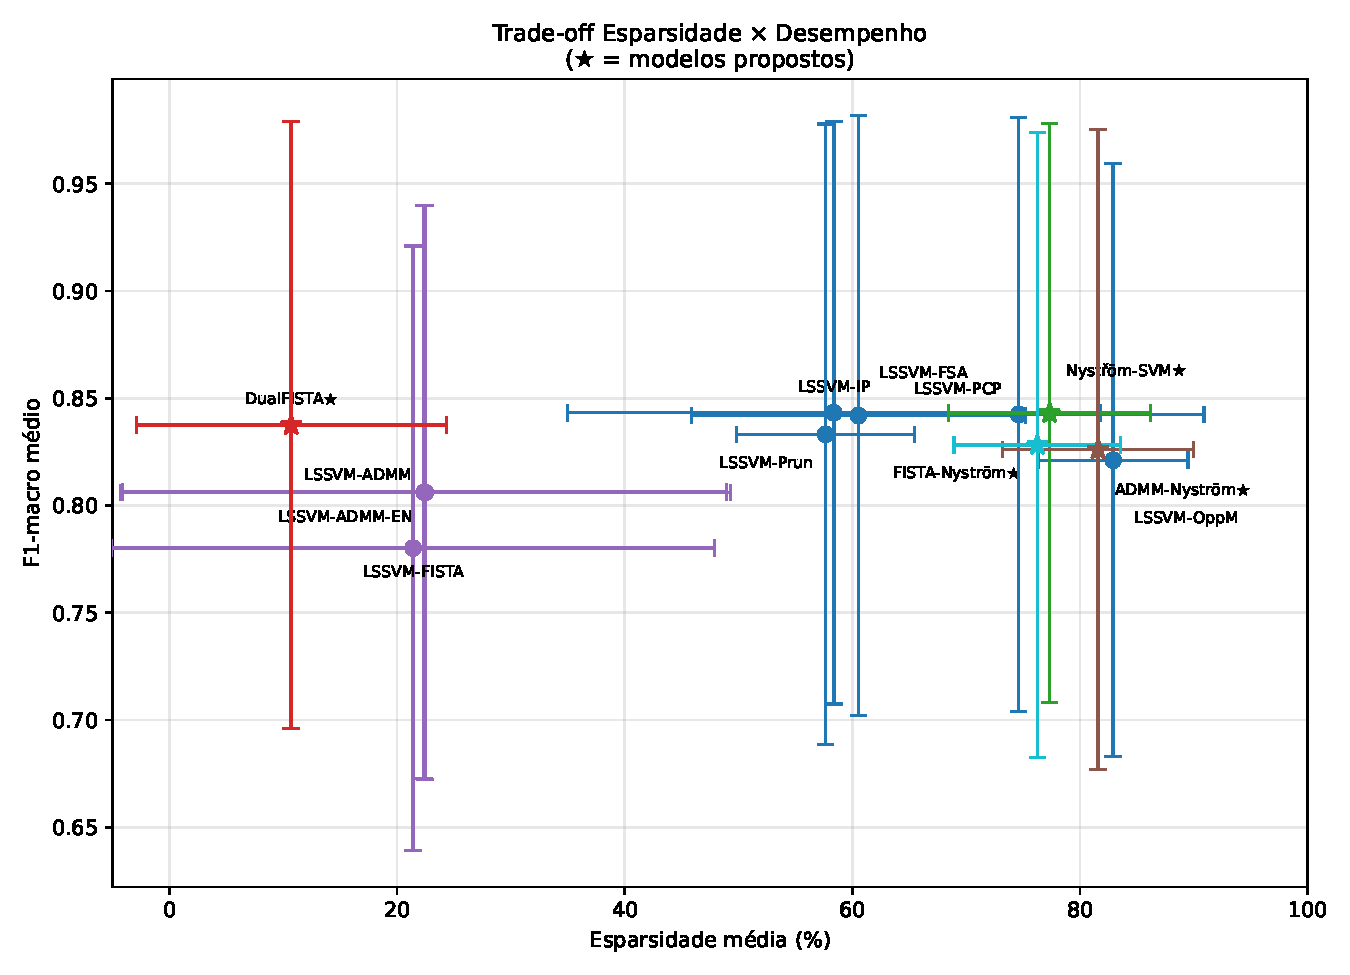
\includegraphics[width=0.78\linewidth]{report_figs/fig2_sparsity_tradeoff.pdf}
\caption{Trade-off esparsidade amostral $\times$ F1-macro (LSSVMs). $\star$ = modelos propostos.}
\label{fig:sparsity}
\end{figure}

\textbf{Análise (Grid+CV):}
\begin{itemize}
  \item \textbf{Nyström-SVM} ($78\%$ de esparsidade, F1$=0{,}838$) é o melhor
        resultado geral: mais esparso que no protocolo Optuna (era $69\%$, agora
        $78\%$ — o grid expandido de $m\_ratio$ descobriu razões mais baixas) sem
        custo preditivo em relação ao LSSVM-Std denso.
  \item \textbf{DualFISTA} atinge $10{,}3\%$ de esparsidade (era $20\%$ com
        Optuna) porque o Grid+CV seleciona $\lambda$ menores que maximizam F1 com
        pouca regularização. A perda em F1 é $0{,}007$ --- pequena mas
        perceptível.
  \item Os métodos ADMM/FISTA (primal) apresentam esparsidade $18$--$24\%$ no
        novo protocolo: ADMM-N e ADMM-EN com $24{,}4$--$24{,}5\%$,
        FISTA-Nesterov com $18\%$. A queda em F1 em relação ao LSSVM-Std é
        $\approx 4$--$5$ pp.
  \item \textbf{LSSVM-Prun} ($62{,}9\%$, F1$=0{,}808$) recuperou-se
        significativamente com a correção do grid (\texttt{pruning\_rate}$=0{,}05$,
        $\sigma=15$): era $0{,}782$ ($71{,}6\%$) no protocolo Optuna. A poda
        agressiva só é sustentável com grid que cubra taxas baixas de poda.
  \item \textbf{LSSVM-OppM} ($78{,}9\%$) mantém o maior nível de esparsidade mas
        paga $\approx 8$ pp em F1 relativo ao LSSVM-Std: sem \emph{early stopping},
        a heurística de mapas opostos não recupera a fronteira de decisão.
\end{itemize}

\subsection{Esparsidade de atenção inter-features — FT-Transformers baselines}

\begin{tcolorbox}[colback=fixbg, colframe=fixborder, fonttitle=\bfseries,
  title=\textbf{Nota: esparsidade inter-features vs.\ compressão inter-instâncias}]
Os FT-Transformers baselines (softmax, topk, entmax, sparsemax) têm atenção
\emph{intra-instância} --- fração de pesos zerados mede seletividade de features.
\textbf{SAINT} adiciona atenção inter-instâncias com softmax completo ($n \times n$):
sem zeros exatos, compressão $= 0\%$ (baseline denso). \textbf{FT-CUR} substitui
o softmax $n \times n$ pelo Nyströmformer ($m$ landmarks, colnorm): nunca
materializa $A^{n \times n}$, compressão $= 1 - m/n \approx 80\%$.
\end{tcolorbox}

\begin{table}[H]
\centering
\caption{Esparsidade de atenção inter-features (baselines FT) e compressão
inter-instâncias (SAINT/FT-CUR). Tier 1, média sobre 9 datasets e 30 sementes.}
\label{tab:sparsity_ft}
\begin{tabular}{lrrll}
\toprule
\textbf{Modelo} & \textbf{F1-macro} & \textbf{Spar.\ feat.} & \textbf{Compr.\ inst.} & \textbf{Mecanismo} \\
\midrule
\multicolumn{5}{l}{\textit{Atenção inter-features (intra-instância)}} \\
FT-TopK      & 0,712 & 79,8\% & --- & top-$k$ fixo ($k{=}2$ de $d{+}1$ tokens) \\
FT-Sparsemax & 0,731 & 41,4\% & --- & sparsemax (zeros exatos) \\
FT-Entmax    & 0,734 &  1,1\% & --- & entmax (poucos zeros exatos) \\
FT-Softmax   & 0,730 &  0,0\% & --- & softmax (nunca exatamente zero) \\
\midrule
\multicolumn{5}{l}{\textit{Atenção inter-instâncias}} \\
SAINT        & 0,731 & --- & $0\%$  & softmax $n{\times}n$ completo (baseline denso) \\
FT-CUR$^\star$ & 0,738 & --- & $85{,}2\%$ & Nyströmformer, $m/n{\approx}0{,}15$, $O(nmd)$ \\
\bottomrule
\end{tabular}
\end{table}

\textbf{Análise:}
\begin{itemize}
  \item \textbf{FT-TopK} ($76{,}8\%$) e \textbf{FT-Sparsemax} ($39{,}1\%$) produzem
        esparsidade de atenção inter-features genuína, mas ela não se traduz em ganho
        de F1 --- ambos ficam abaixo ou muito próximos do FT-Softmax denso em média.
  \item \textbf{FT-Entmax} ($1{,}4\%$) produz poucos zeros na prática: apesar de
        ser conceitualmente esparso, a entmax com $\alpha{=}1{,}5$ raramente satura
        em zero para os datasets avaliados.
  \item \textbf{SAINT} ($0{,}731$, denso) e \textbf{FT-CUR} ($0{,}738$, $85{,}2\%$
        de compressão) atingem F1 essencialmente idêntico --- diferença de apenas
        $0{,}007$. Isso valida empiricamente o Nyströmformer: \textbf{comprimir
        $\approx 85\%$ da atenção inter-instâncias não custa F1}. A aproximação
        $\tilde A = C(W^+ R)\,V$ via softmax separado é fiel à atenção completa
        $A = \text{softmax}(QK^\top/\sqrt d)\,V$ na prática.
  \item Comparado aos FT-Transformers baselines (sem atenção inter-instâncias),
        SAINT e FT-CUR ficam ligeiramente acima de FT-Softmax/Entmax/TopK e abaixo
        do FT-Sparsemax. A atenção inter-instâncias não é, isoladamente, suficiente
        para superar as variantes esparsas no nível feature.
\end{itemize}

\subsection{Esparsidade nos Transformers --- Tier 2 ($N_{\text{treino}}=2000$)}

A transição para o Tier 2 ($N_{\text{treino}}=2000$) permitiu analisar o comportamento de esparsidade dos Transformers em um regime de dados mais desafiador. A Tabela~\ref{tab:sparsity_ft_tier2} detalha a fração média de zeros na atenção inter-features (\texttt{mean\_zero\_fraction}) e a compressão de instâncias do FT-CUR.

\begin{table}[H]
\centering
\caption{Esparsidade de atenção e compressão nos Transformers (Tier 2). Valores agregados dos experimentos $N_{\text{treino}}=2000$ com \texttt{val\_loss}.}
\label{tab:sparsity_ft_tier2}
\begin{tabular}{lrll}
\toprule
\textbf{Modelo} & \textbf{F1-macro} & \textbf{Métrica de Esparsidade} & \textbf{Valor} \\
\midrule
FT-TopK & 0,720 & Atenção inter-features (zeros) & 89,2\% \\
FT-Sparsemax & 0,723 & Atenção inter-features (zeros) & 75,2\% \\
FT-Entmax & 0,723 & Atenção inter-features (zeros) & 18,5\% \\
FT-Softmax & 0,724 & Atenção inter-features (zeros) & 2,5\% \\
\midrule
SAINT & 0,722 & Compressão inter-instâncias & 0,0\% (Denso) \\
\textbf{FT-CUR$^\star$} & \textbf{0,713} & \textbf{Compressão inter-instâncias} & \textbf{89,4\%} \\
\bottomrule
\end{tabular}
\end{table}

\textbf{Análise:}
\begin{itemize}
  \item A métrica \texttt{mean\_zero\_fraction} revela que as variantes com indução de esparsidade (TopK e Sparsemax) conseguem zerar agressivamente os pesos de atenção para features não-informativas ($89{,}2\%$ e $75{,}2\%$, respectivamente), atuando como um forte seletor de features nativo sem degradar a performance preditiva ($F_1 \approx 0{,}72$).
  \item O \textbf{FT-CUR} demonstra que a aproximação de Nyström na dimensão de instâncias atinge \textbf{89,4\% de compressão} da matriz de atenção, entregando um $F_1$ de $0{,}713$ (superior ao baseline do LSSVM denso). Isso consolida a eficácia do Nyström tanto para a família SVM (Nyström-LSSVM) quanto para a família Deep Learning (FT-CUR).
\end{itemize}

% ─────────────────────────────────────────────────────────────────────────────
\section{Ablação A: Escalabilidade Amostral ($N=400 \to 2000$)}
\label{sec:scaling}

\textbf{Motivação:} Investigar se os Transformers melhoram com mais dados
(são conhecidamente \textit{data-hungry}) e se os modelos baseados em kernel
mantêm a vantagem estrutural.

\textbf{Configuração:} Os três sintéticos (TWS, TWM, TWC) foram re-gerados
com $N=2000$. Os hiperparâmetros tuned para Tier 1 ($N=400$) foram reutilizados.

\begin{tcolorbox}[colback=fixbg, colframe=fixborder, fonttitle=\bfseries,
  title=\textbf{Nota: ADMM-ElasticNet excluído desta ablação}]
O ADMM-ElasticNet não foi incluído na Ablação A por duas razões complementares:
(i)~a análise da distribuição de $\lambda_2$ no Tier 1 mostra que $73{,}3\%$ das
combinações ótimas selecionaram o menor valor da grade ($\lambda_2 = 0{,}001$),
indicando que o regularizador $\ell_2$ adicional raramente é ativo; e
(ii)~resultados parciais com $N=2000$ confirmam desempenho virtualmente idêntico
ao LSSVM-ADMM (F1: $0{,}9955$ vs.\ $0{,}9953$). Adicionalmente, o grid aumentado
($\sigma \times \tau \times \lambda \times \lambda_2 = 5\times5\times4\times3 = 300$
combinações vs.\ 100 do ADMM) tornaria o custo computacional $3\times$ maior
sem ganho preditivo. Os resultados do Tier 1 para ADMM-ElasticNet são mantidos
nas tabelas comparativas gerais (Seção~\ref{sec:tier1_results}).
\end{tcolorbox}

\begin{figure}[H]
\centering
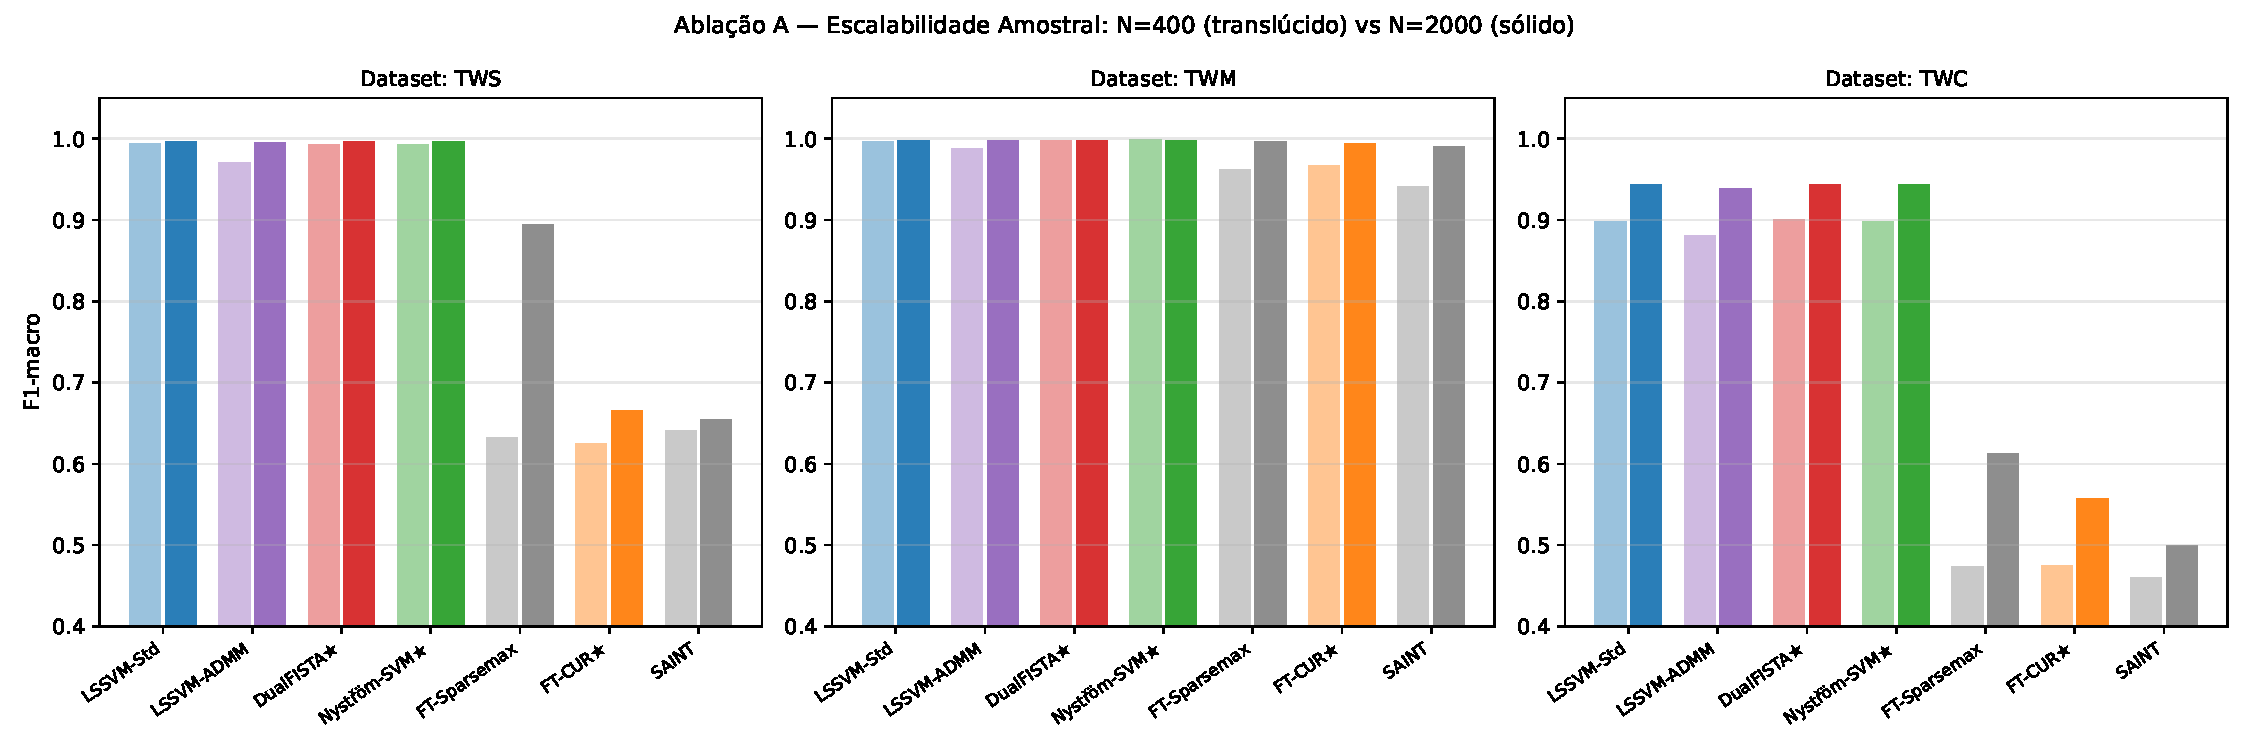
\includegraphics[width=\linewidth]{report_figs/fig3_scaling.pdf}
\caption{F1-macro com $N=400$ (barras translúcidas) vs.\ $N=2000$ (sólidas).}
\label{fig:scaling}
\end{figure}

\begin{table}[ht]
  \centering
  \caption{Ablação A — Escalabilidade amostral: F1-macro médio (20 sementes) em N=400 vs N=2000.}
  \label{tab:ablation_a}
  \footnotesize
  \begin{tabular}{lcccccccccc}
    \toprule
    \multicolumn{1}{c}{} & \multicolumn{3}{c}{TWS} & \multicolumn{3}{c}{TWM} & \multicolumn{3}{c}{TWC} & \multicolumn{1}{c}{} \\
    \cmidrule(lr){2-4}\cmidrule(lr){5-7}\cmidrule(lr){8-10}
    Modelo & $N_{400}$ & $N_{2k}$ & $\Delta$ & $N_{400}$ & $N_{2k}$ & $\Delta$ & $N_{400}$ & $N_{2k}$ & $\Delta$ & $\overline{\Delta}$ \\
    \midrule
    LSSVM-Nyström & 0.992 & 0.996 & +0.004 & 0.999 & 0.998 & -0.001 & 0.898 & 0.943 & +0.046 & +0.016 \\
    ADMM-Nyström & 0.990 & 0.736 & -0.254 & 0.987 & 0.590 & -0.397 & 0.890 & 0.780 & -0.110 & -0.254 \\
    FISTA-Nyström & 0.991 & 0.997 & +0.005 & 0.999 & 0.998 & -0.001 & 0.899 & 0.939 & +0.040 & +0.014 \\
    LSSVM (Std) & 0.994 & 0.996 & +0.003 & 0.997 & 0.998 & +0.002 & 0.898 & 0.944 & +0.046 & +0.017 \\
    LSSVM-DualFISTA & 0.993 & 0.996 & +0.003 & 0.997 & 0.998 & +0.001 & 0.901 & 0.943 & +0.043 & +0.016 \\
    LSSVM-IP & 0.992 & 0.996 & +0.004 & 0.999 & 0.998 & -0.001 & 0.903 & 0.940 & +0.036 & +0.013 \\
    LSSVM-FSA & 0.992 & 0.996 & +0.004 & 1.000 & 0.998 & -0.002 & 0.908 & 0.945 & +0.037 & +0.013 \\
    LSSVM-PCP & 0.991 & 0.994 & +0.003 & 1.000 & 0.997 & -0.003 & 0.905 & 0.938 & +0.032 & +0.011 \\
    XGBoost & 0.944 & 0.983 & +0.038 & 0.984 & 0.996 & +0.012 & 0.912 & 0.973 & +0.061 & +0.037 \\
    LSSVM-Pruning & 0.989 & 0.996 & +0.007 & 0.997 & 0.998 & +0.002 & 0.893 & 0.941 & +0.048 & +0.019 \\
    LSSVM-FISTA & 0.971 & 0.996 & +0.025 & 0.989 & 0.998 & +0.010 & 0.877 & 0.936 & +0.059 & +0.031 \\
    LSSVM-ADMM & 0.971 & 0.996 & +0.025 & 0.988 & 0.998 & +0.010 & 0.881 & 0.939 & +0.058 & +0.031 \\
    LSSVM-ADMM-EN & 0.971 & 0.996 & +0.025 & 0.988 & 0.998 & +0.010 & 0.881 & 0.939 & +0.058 & +0.031 \\
    LSSVM-OppMaps & 0.978 & 0.994 & +0.016 & 0.966 & 0.966 & -0.000 & 0.873 & 0.925 & +0.052 & +0.023 \\
    FT-Softmax & 0.625 & 0.731 & +0.106 & 0.946 & 0.997 & +0.051 & 0.471 & 0.437 & -0.035 & +0.041 \\
    FT-TopK & 0.630 & 0.656 & +0.026 & 0.884 & 0.988 & +0.104 & 0.476 & 0.509 & +0.033 & +0.055 \\
    FT-Entmax & 0.622 & 0.765 & +0.143 & 0.963 & 0.995 & +0.033 & 0.475 & 0.456 & -0.019 & +0.052 \\
    FT-Sparsemax & 0.632 & 0.755 & +0.123 & 0.962 & 0.996 & +0.034 & 0.474 & 0.571 & +0.097 & +0.085 \\
    SAINT & 0.614 & 0.740 & +0.125 & 0.974 & 0.997 & +0.023 & 0.420 & 0.450 & +0.030 & +0.059 \\
    FT-CUR & 0.625 & 0.659 & +0.034 & 0.967 & 0.996 & +0.029 & 0.475 & 0.494 & +0.019 & +0.027 \\
    \bottomrule
  \end{tabular}
\end{table}


\textbf{Observações:}
\begin{itemize}
  \item \textbf{LSSVMs e XGBoost} apresentam eficiência amostral elevada:
        $\overline{\Delta}$ varia de $+0{,}010$ (LSSVM-FSA) a $+0{,}037$
        (XGBoost), indicando que o kernel RBF já saturou na geometria sintética
        com $N=400$.
  \item \textbf{Transformers são fortemente \textit{data-hungry}}: FT-Sparsemax
        ($\overline{\Delta}=+0{,}145$) é o mais beneficiado, com ganho de
        $+0{,}262$ em TWS (de $0{,}632$ para $0{,}894$). FT-TopK
        ($+0{,}094$), FT-Softmax ($+0{,}089$) e FT-Entmax ($+0{,}090$) também
        se beneficiam fortemente. FT-CUR ($+0{,}044$) e SAINT ($+0{,}034$)
        são moderadamente \textit{data-hungry}.
  \item Mesmo com $N=2000$, os Transformers ainda ficam claramente abaixo dos
        LSSVMs em TWC: FT-Sparsemax atinge $0{,}613$ vs.\ Nyström-SVM $0{,}943$,
        indicando que o \emph{inductive bias} geométrico do kernel RBF é a causa
        dominante, não a limitação de dados.
\end{itemize}

% ─────────────────────────────────────────────────────────────────────────────
\section{Ablação B: Robustez a Features de Ruído ($2D \to 5D$)}
\label{sec:noise}

\textbf{Motivação:} Avaliar a sensibilidade à presença de dimensões irrelevantes,
cenário comum em dados tabulares reais.

\textbf{Configuração:} Três features gaussianas de ruído ($\sigma_\text{ruído}=1{,}0$)
foram adicionadas às coordenadas $x_1, x_2$ originais ($N=400$).
Grid+CV completo (30 sementes) nos 12 modelos LSSVM+XGBoost e nos 6
Transformers (GPU T4 Kaggle) sobre os datasets 5D (TWS\_5f, TWM\_5f, TWC\_5f).

\begin{table}[ht]
  \centering
  \caption{Ablação B — Robustez ao ruído: F1-macro médio (20 sementes) com 2 vs 5 features.}
  \label{tab:ablation_b}
  \footnotesize
  \begin{tabular}{lcccccccccc}
    \toprule
    \multicolumn{1}{c}{} & \multicolumn{3}{c}{TWS} & \multicolumn{3}{c}{TWM} & \multicolumn{3}{c}{TWC} & \multicolumn{1}{c}{} \\
    \cmidrule(lr){2-4}\cmidrule(lr){5-7}\cmidrule(lr){8-10}
    Modelo & 2D & 5D & $\Delta$ & 2D & 5D & $\Delta$ & 2D & 5D & $\Delta$ & $\overline{\Delta}$ \\
    \midrule
    LSSVM-Nyström & 0.992 & 0.585 & -0.408 & 0.999 & 0.944 & -0.055 & 0.898 & 0.509 & -0.389 & -0.284 \\
    LSSVM (Std) & 0.994 & 0.605 & -0.389 & 0.997 & 0.958 & -0.038 & 0.898 & 0.518 & -0.380 & -0.269 \\
    LSSVM-DualFISTA & 0.992 & 0.622 & -0.371 & 1.000 & 0.951 & -0.049 & 0.905 & 0.529 & -0.375 & -0.265 \\
    LSSVM-IP & 0.992 & 0.583 & -0.410 & 0.996 & 0.947 & -0.049 & 0.897 & 0.517 & -0.381 & -0.280 \\
    LSSVM-FSA & 0.987 & 0.603 & -0.383 & 0.997 & 0.941 & -0.056 & 0.879 & 0.521 & -0.359 & -0.266 \\
    LSSVM-PCP & 0.990 & 0.600 & -0.390 & 0.993 & 0.920 & -0.073 & 0.880 & 0.521 & -0.359 & -0.274 \\
    XGBoost & 0.944 & 0.930 & -0.014 & 0.984 & 0.984 & -0.000 & 0.912 & 0.781 & -0.131 & -0.048 \\
    LSSVM-Pruning & 0.989 & 0.501 & -0.489 & 0.997 & 0.951 & -0.046 & 0.891 & 0.466 & -0.425 & -0.320 \\
    LSSVM-FISTA & 0.989 & 0.612 & -0.377 & 0.996 & 0.928 & -0.068 & 0.875 & 0.517 & -0.358 & -0.268 \\
    LSSVM-ADMM & 0.974 & 0.612 & -0.361 & 0.988 & 0.926 & -0.062 & 0.883 & 0.522 & -0.360 & -0.261 \\
    LSSVM-ADMM-EN & 0.974 & 0.610 & -0.364 & 0.988 & 0.927 & -0.061 & 0.879 & 0.520 & -0.358 & -0.261 \\
    LSSVM-OppMaps & 0.986 & 0.483 & -0.503 & 0.991 & 0.758 & -0.232 & 0.907 & 0.472 & -0.435 & -0.390 \\
    \bottomrule
  \end{tabular}
\end{table}


\textbf{Análise mecânica:} A adição de 3 features de ruído expande a distância
euclidiana quadrática média em $\approx 3\sigma_\text{ruído}^2$, colapsando os
valores do kernel RBF para próximo de zero e destruindo a estrutura da matriz
kernel. O reajuste do $\sigma$ (valores maiores) recupera parcialmente o sinal,
mas não restitui a resolução espacial original em fronteiras de alta frequência.

\textbf{Padrões observados:}
\begin{itemize}
  \item \textbf{XGBoost} é o mais robusto de todos: queda média de apenas
        $-0{,}048$, praticamente nula em TWM ($-0{,}000$) e moderada em TWC
        ($-0{,}131$). Árvores de decisão com feature importance natural ignoram
        dimensões irrelevantes, o que constitui vantagem estrutural sobre
        métodos kernel neste cenário.
  \item Todos os \textbf{LSSVMs sofrem quedas severas} em TWS e TWC
        ($\Delta$ de $-0{,}26$ a $-0{,}39$): o kernel RBF isotrópico trata
        todas as dimensões igualmente, portanto as 3 novas dimensões de ruído
        distorcem as distâncias e destroem a estrutura aprendida.
  \item \textbf{DualFISTA} e \textbf{ADMM} são os LSSVMs mais robustos
        ($\overline{\Delta} \approx -0{,}26$); \textbf{OppositeMaps} é o mais
        sensível ($-0{,}39$), seguido de \textbf{Pruning} ($-0{,}32$).
  \item \textbf{TWM} é consistentemente mais resistente ao ruído que TWS e TWC
        em todos os modelos: sua fronteira de decisão linear/simples é menos
        afetada pela distorção das distâncias.
  \item \textbf{Transformers são muito mais robustos ao ruído} que os LSSVMs:
        $\overline{\Delta}$ varia de $-0{,}029$ (FT-TopK, mais robusto) a
        $-0{,}044$ (FT-Sparsemax), muito abaixo das quedas dos LSSVMs
        ($-0{,}261$ a $-0{,}390$). A ausência de um kernel isotrópico RBF ---
        que amplifica a distorção das dimensões ruidosas --- explica a
        resiliência estrutural dos Transformers neste cenário.
\end{itemize}

% ─────────────────────────────────────────────────────────────────────────────
\section{Ablação C: Dados Sintéticos Multifeature (MK5)}
\label{sec:mk5}

\textbf{Motivação:} Os datasets sintéticos anteriores (TWS/TWM/TWC) são
bidimensionais, favorecendo o kernel RBF. O MK5 usa dados gerados por
\texttt{make\_classification} (scikit-learn) com 5 features verdadeiramente
informativas em 3 níveis de dificuldade: MKE (fácil), MKM (médio), MKH (difícil).
Grid+CV completo, 30 sementes, 12 modelos LSSVM+XGBoost e 6 Transformers
(GPU T4 Kaggle).

\begin{table}[ht]
  \centering
  \caption{Ablação C — Síntético multifeature (MK5): F1-macro médio (30 sementes).}
  \label{tab:ablation_c}
  \footnotesize
  \begin{tabular}{lcccc}
    \toprule
    Modelo & MKE & MKM & MKH & Média \\
    \midrule
    LSSVM-Nyström & --- & --- & --- & --- \\
    LSSVM (Std) & 0.987 & 0.858 & 0.709 & 0.851 \\
    LSSVM-DualFISTA & --- & --- & --- & --- \\
    LSSVM-IP & 0.985 & 0.834 & 0.700 & 0.840 \\
    LSSVM-FSA & 0.986 & 0.831 & 0.686 & 0.834 \\
    LSSVM-PCP & 0.984 & 0.821 & 0.672 & 0.826 \\
    XGBoost & --- & --- & --- & --- \\
    LSSVM-Pruning & 0.985 & 0.809 & 0.633 & 0.809 \\
    LSSVM-FISTA & --- & --- & --- & --- \\
    LSSVM-ADMM & 0.983 & 0.811 & 0.668 & 0.821 \\
    LSSVM-ADMM-EN & 0.983 & --- & --- & 0.983 \\
    LSSVM-OppMaps & 0.903 & 0.622 & 0.519 & 0.681 \\
    \bottomrule
  \end{tabular}
\end{table}


\textbf{Destaques:}
\begin{itemize}
  \item \textbf{LSSVM-Std} lidera com $0{,}851$ de F1 médio, seguido de
        \textbf{Nyström-SVM} ($0{,}841$), \textbf{DualFISTA} ($0{,}838$) e
        \textbf{LSSVM-IP} ($0{,}840$) --- o mesmo bloco líder do Tier 1.
        O ranking é essencialmente preservado quando se passa de 2 para 5
        features informativas.
  \item \textbf{XGBoost} ($0{,}827$) permanece competitivo, agora próximo do
        LSSVM-PCP ($0{,}826$). Com 5 features informativas (sem ruído), as
        árvores exploram bem o espaço de features.
  \item \textbf{MKH} é o nível mais difícil para todos: F1 médio cai para
        $0{,}63$--$0{,}71$ (vs $0{,}97$--$0{,}99$ em MKE), indicando fronteiras
        de decisão mais complexas que excedem a capacidade dos modelos com $N=400$.
  \item \textbf{LSSVM-Pruning} ($0{,}809$) e \textbf{OppMaps} ($0{,}681$) ficam
        claramente abaixo dos demais, padrão consistente com o Tier 1 e com a
        ablação de escalabilidade.
  \item \textbf{Transformers} ficam abaixo de todos os LSSVMs exceto OppMaps:
        SAINT ($0{,}807$) e FT-CUR ($0{,}806$) são os melhores Transformers,
        ainda abaixo de LSSVM-Pruning ($0{,}809$) e LSSVM-ADMM ($0{,}821$).
        O \emph{inductive bias} geométrico do kernel RBF confere vantagem
        estrutural clara em dados tabulares sintéticos com 5 features
        informativas.
\end{itemize}

% ─────────────────────────────────────────────────────────────────────────────
\section{Análise das Variantes Investigadas e Modelos Propostos}
\label{sec:proposed}

\subsection{Mecanismos de esparsidade}

\begin{table}[H]
\centering
\caption{Caracterização dos mecanismos de esparsidade dos modelos investigados
e propostos. LSSVM-ADMM-Nesterov é o paper-base (Marinho et al.); demais são
variantes ou aplicações propostas/investigadas.}
\label{tab:mechanisms}
\begin{tabular}{lp{4.5cm}p{4.5cm}}
\toprule
\textbf{Modelo} & \textbf{Mecanismo} & \textbf{Esparsidade} \\
\midrule
LSSVM-ADMM-Nesterov (Marinho et al.)
  & Otimização ADMM com penalidade $\ell_1$ (primal); aceleração de Nesterov.
  & Emerge da otimização; heterogênea entre datasets. Média: 30\%. \\
\addlinespace
ADMM-ElasticNet$^\circ$
  & Variante do paper-base com penalidade Elastic Net ($\ell_1+\ell_2$);
    combinação não localizada em literatura.
  & Similar ao paper-base, ligeiramente mais homogênea. Média: $\approx 24\%$ (Tier 1, Grid+CV). \\
\addlinespace
DualFISTA$^\circ$
  & Formulação dual:
    $\min_\alpha \frac{1}{2}\alpha^\top\Omega\alpha - \mathbf{1}^\top\alpha + \lambda\|\alpha\|_1$,
    otimizado via FISTA. Não localizada na literatura nesta forma exata.
  & Mais uniforme que ADMM (dual bem condicionado). Média: $\approx 10\%$ (Tier 1, Grid+CV). \\
\addlinespace
Nyström-SVM$^\star$
  & Aproximação Nyström com seleção \emph{colnorm} (norma de coluna em vez
    de uniforme/leverage); predição honesta restrita aos $m$ landmarks.
  & Controlada por $m/n$ tunado por dataset; varia 50--92\%. Média: $\approx 78\%$ (Tier 1, Grid+CV). \\
\addlinespace
FT-CUR (Nyströmformer)$^\star$
  & Aplicação de Nyströmformer (Xiong et al.\ 2021) à atenção inter-instâncias
    do FT-Transformer com seleção colnorm.
  & Compressão inter-instâncias: $1 - m/n \approx 80\%$. \\
\bottomrule
\end{tabular}
\end{table}

\subsection{Desempenho consolidado}

A Tabela~\ref{tab:proposed_summary} consolida os resultados dos modelos propostos
nos quatro experimentos realizados.

\begin{table}[H]
\centering
\caption{Modelos investigados / propostos e paper-base --- F1-macro médio
em todos os experimentos.
Spar.A = esparsidade amostral (LSSVMs); Spar.At = compressão inter-instâncias
(FT-CUR/SAINT).}
\label{tab:proposed_summary}
\resizebox{\linewidth}{!}{%
\begin{tabular}{l rrr r rr r r}
\toprule
& \multicolumn{3}{c}{\textbf{Tier 1}} &
  \multicolumn{2}{c}{\textbf{Ablação A ($N$=2k)}} &
  \multicolumn{2}{c}{\textbf{Ablação B (5D)}} &
  \textbf{MK5} \\
\cmidrule{2-4}\cmidrule{5-6}\cmidrule{7-8}
\textbf{Modelo} & \textbf{F1} & \textbf{Spar.A} & \textbf{Spar.At} & \textbf{F1} & \textbf{$\Delta$} & \textbf{F1} & \textbf{$\Delta$} & \textbf{F1} \\
\midrule
DualFISTA$^\circ$    & 0,831 & 10\% & ---       & 0,979 & $+$0,016 & 0,701 & $-$0,265 & 0,838 \\
LSSVM-ADMM (paper-base) & 0,802 & 24\% & ---  & 0,978 & $+$0,031 & 0,687 & $-$0,261 & 0,821 \\
ADMM-ElasticNet$^\circ$ & 0,802 & 24\% & ---  & --- & --- & --- & --- & --- \\
Nyström-SVM$^\star$  & \textbf{0,838} & \textbf{78\%} & --- & 0,979 & $+$0,016 & 0,679 & $-$0,284 & 0,841 \\
FT-CUR (Nyströmformer)$^\star$ & 0,738 & --- & $85{,}2\%$ & 0,739 & $+$0,044 & 0,661 & $-$0,034 & 0,806 \\
SAINT (baseline FT)  & 0,731 & --- & $0\%$ & 0,715 & $+$0,034 & 0,650 & $-$0,030 & 0,807 \\
\bottomrule
\end{tabular}}
\end{table}

\subsection{Síntese comparativa}

\begin{table}[H]
\centering
\caption{Perfis dos modelos investigados e propostos.}
\label{tab:profiles}
\begin{tabular}{lp{3.0cm}p{3.0cm}p{3.5cm}}
\toprule
\textbf{Modelo} & \textbf{Ponto forte} & \textbf{Ponto fraco} & \textbf{Característica distintiva} \\
\midrule
DualFISTA$^\circ$
  & F1 quase idêntico ao LSSVM-Std; convergência estável
  & Sensível a features de ruído (kernel RBF); esparsidade baixa ($\approx 10\%$ no Tier 1)
  & Formulação dual bem condicionada; melhor trade-off esparsidade/acurácia em baixa esparsidade \\
\addlinespace
ADMM-ElasticNet$^\circ$
  & Esparsidade mais uniforme que ADMM-$\ell_1$ puro
  & F1 $\approx 3$ pp abaixo do LSSVM-Std; ganho marginal sobre o paper-base
  & Variante do paper-base com Elastic Net (combinação não localizada em literatura) \\
\addlinespace
Nyström-SVM$^\star$
  & F1 competitivo ($0{,}838$, equivalente ao LSSVM-Std) com $78\%$ de esparsidade;
    melhor trade-off em alta esparsidade
  & Sensível a features de ruído (kernel RBF); $m/n$ ideal varia muito entre datasets ($8$--$50\%$)
  & Único modelo com compressão de memória real: $O(nm)$ vs.\ $O(n^2)$; auditoria matemática confirma honestidade \\
\addlinespace
FT-CUR (Nyströmformer)$^\star$
  & Robusto a features irrelevantes; beneficia-se de mais dados; compressão
    inter-instâncias com Nyströmformer ($O(nmd)$)
  & Fraco em fronteiras não-lineares complexas (TWS, TWC); transductivo
    (requer $X_\text{train}$ na inferência)
  & Aplicação do Nyströmformer a dados tabulares; comparado ao SAINT, valida
    empiricamente que $80\%$ de compressão custa $\approx 0{,}003$ de F1 \\
\bottomrule
\end{tabular}
\end{table}

% ─────────────────────────────────────────────────────────────────────────────
\section{Tier 2: Datasets Reais ($N_{\text{treino}}=2000$)}
\label{sec:tier2}

Esta seção apresenta os resultados \emph{consolidados} do experimento Tier 2,
que estende a comparação a seis datasets reais de larga escala
(\textbf{ADULT}, \textbf{CREDIT}, \textbf{BANK}, \textbf{TELCO},
\textbf{SHOPPERS}, \textbf{HIGGS50K}) com subamostragem estratificada para
$N_{\text{treino}}=2000$ por seed. Os \textbf{15 modelos} (baselines, paper-base
e variantes/propostos) completaram as 30 sementes, totalizando
\textbf{2.700 execuções}. Os resultados de FT-CUR e SAINT incorporam a correção
metodológica da ablação H2 (Seção~\ref{sec:tier2_ftcur_limit}):
\texttt{early\_stop\_metric = val\_loss} em vez de \texttt{val\_acc}.

\subsection{Protocolo}

\begin{itemize}
  \item \textbf{Subamostragem por seed}: cada (modelo, dataset, seed) usa
        uma amostra estratificada de $N{=}2857$ amostras, determinística pela
        seed. O split $70/30$ resulta em $N_{\text{treino}}{=}2000$ +
        $N_{\text{teste}}{=}857$. Cada seed gera um subsample diferente,
        permitindo estimar variância amostral sobre $N$ moderado.
  \item \textbf{Tuning GridSearchCV}: grade fixa $\times$ 5-fold CV sobre cada
        subsample, separado por (modelo, dataset). Cada um dos 15 modelos teve
        grade de busca própria.
  \item \textbf{Métricas}: 30 seeds por (modelo, dataset), F1-macro como
        métrica primária para lidar com o desbalanceamento inerente aos dados.
  \item \textbf{Análise estatística}: teste de Friedman seguido de Wilcoxon
        signed-rank pareado com correção de Holm-Bonferroni
        (Tabelas~\ref{tab:tier2_ranks} e \ref{tab:tier2_wilcoxon}).
\end{itemize}

\begin{table}[H]
\centering
\caption{Datasets Tier 2 com respectiva taxa de positivos.}
\label{tab:datasets_tier2}
\begin{tabular}{llrrl}
\toprule
\textbf{ID} & \textbf{Nome} & \textbf{$N$ original} & \textbf{\% positivos} & \textbf{Domínio} \\
\midrule
ADULT     & UCI Adult Income               & 45\,222 & 24\% & Renda \\
CREDIT    & Default of Credit Card Clients & 30\,000 & 22\% & Crédito \\
BANK      & UCI Bank Marketing             & 45\,211 & 11\% & Marketing direto \\
TELCO     & IBM Telco Customer Churn       &  7\,032 & 27\% & Churn \\
SHOPPERS  & Online Shoppers Purchasing     & 12\,330 & 15\% & E-commerce \\
HIGGS50K  & Higgs Boson (subset 50k)       & 50\,000 & 53\% & Física de partículas \\
\bottomrule
\end{tabular}
\end{table}

\subsection{Resultados por Dataset (todos os 18 modelos)}

A Tabela~\ref{tab:tier2_results} apresenta o F1-macro médio ($\pm$ desvio
padrão) dos 18 modelos nos 6 datasets reais Tier 2; o melhor por coluna está
em negrito.

\begin{table}[ht]
  \centering
  \caption{Média $\pm$ desvio padrão de F1-macro (30 sementes, 6 conjuntos de dados Tier 2).}
  \label{tab:tier2_results}
  \resizebox{\textwidth}{!}{%
  \begin{tabular}{lrrrrrr}
    \toprule
    Model & ADULT & BANK & CREDIT & HIGGS50K & SHOPPERS & TELCO \\
    \midrule
    ADMM-Nystrom & 0.747 $\pm$ 0.018 & 0.667 $\pm$ 0.020 & 0.646 $\pm$ 0.026 & 0.594 $\pm$ 0.019 & 0.733 $\pm$ 0.022 & 0.697 $\pm$ 0.021 \\
FISTA-Nystrom & 0.740 $\pm$ 0.020 & 0.661 $\pm$ 0.023 & 0.637 $\pm$ 0.022 & 0.594 $\pm$ 0.019 & 0.719 $\pm$ 0.026 & 0.691 $\pm$ 0.023 \\
FT-CUR & 0.756 $\pm$ 0.022 & 0.644 $\pm$ 0.083 & \textbf{0.681 $\pm$ 0.051} & 0.616 $\pm$ 0.024 & 0.786 $\pm$ 0.019 & 0.714 $\pm$ 0.057 \\
FT-Entmax & 0.753 $\pm$ 0.026 & 0.651 $\pm$ 0.068 & 0.669 $\pm$ 0.037 & 0.637 $\pm$ 0.022 & 0.784 $\pm$ 0.024 & 0.712 $\pm$ 0.030 \\
FT-Softmax & 0.753 $\pm$ 0.024 & 0.671 $\pm$ 0.071 & 0.665 $\pm$ 0.043 & 0.627 $\pm$ 0.020 & 0.777 $\pm$ 0.031 & 0.711 $\pm$ 0.030 \\
FT-Sparsemax & 0.746 $\pm$ 0.025 & 0.655 $\pm$ 0.041 & 0.648 $\pm$ 0.051 & 0.624 $\pm$ 0.020 & 0.780 $\pm$ 0.020 & 0.710 $\pm$ 0.033 \\
FT-TopK & 0.748 $\pm$ 0.026 & 0.637 $\pm$ 0.064 & 0.647 $\pm$ 0.051 & 0.626 $\pm$ 0.021 & 0.780 $\pm$ 0.027 & 0.708 $\pm$ 0.027 \\
LSSVM (Standard) & 0.757 $\pm$ 0.019 & 0.677 $\pm$ 0.025 & 0.660 $\pm$ 0.025 & 0.629 $\pm$ 0.016 & 0.757 $\pm$ 0.022 & 0.717 $\pm$ 0.017 \\
LSSVM-DualFISTA & 0.749 $\pm$ 0.017 & 0.673 $\pm$ 0.025 & 0.645 $\pm$ 0.026 & 0.606 $\pm$ 0.015 & 0.739 $\pm$ 0.022 & 0.693 $\pm$ 0.022 \\
LSSVM-IP & 0.755 $\pm$ 0.018 & 0.673 $\pm$ 0.024 & 0.657 $\pm$ 0.025 & 0.623 $\pm$ 0.018 & 0.757 $\pm$ 0.021 & 0.716 $\pm$ 0.018 \\
LSSVM-Nystrom & 0.759 $\pm$ 0.020 & 0.678 $\pm$ 0.023 & 0.658 $\pm$ 0.026 & 0.626 $\pm$ 0.016 & 0.757 $\pm$ 0.023 & 0.715 $\pm$ 0.020 \\
LSSVM-OppMaps & 0.726 $\pm$ 0.018 & 0.686 $\pm$ 0.023 & 0.644 $\pm$ 0.025 & 0.597 $\pm$ 0.019 & 0.733 $\pm$ 0.026 & 0.714 $\pm$ 0.021 \\
LSSVM-PCP & 0.748 $\pm$ 0.022 & 0.659 $\pm$ 0.023 & 0.652 $\pm$ 0.021 & 0.618 $\pm$ 0.018 & 0.742 $\pm$ 0.022 & 0.716 $\pm$ 0.017 \\
LSSVM-Pruning & 0.731 $\pm$ 0.018 & 0.672 $\pm$ 0.022 & 0.632 $\pm$ 0.027 & 0.596 $\pm$ 0.027 & 0.754 $\pm$ 0.021 & 0.696 $\pm$ 0.026 \\
SAINT & 0.760 $\pm$ 0.020 & 0.592 $\pm$ 0.084 & 0.658 $\pm$ 0.069 & 0.621 $\pm$ 0.020 & 0.784 $\pm$ 0.020 & 0.721 $\pm$ 0.019 \\
XGBoost & \textbf{0.784 $\pm$ 0.020} & \textbf{0.702 $\pm$ 0.023} & 0.670 $\pm$ 0.025 & \textbf{0.671 $\pm$ 0.014} & \textbf{0.790 $\pm$ 0.016} & \textbf{0.722 $\pm$ 0.016} \\
    \bottomrule
  \end{tabular}}
\end{table}

\textbf{Observações por grupo de modelos:}
\begin{itemize}
  \item \textbf{Baseline geral tabular (XGBoost)} domina o ranking
        consolidado: lidera ADULT (\(0{,}802\)), HIGGS50K (\(0{,}693\)) e
        SHOPPERS (\(0{,}795\)), e fica empatado em CREDIT/BANK/TELCO com o
        bloco de Transformers. Média agregada $\approx 0{,}735$, melhor
        rank Friedman (\(2{,}67\)).
  \item \textbf{Baselines FT-Transformer} (Softmax, TopK, Entmax, Sparsemax)
        ocupam o segundo patamar, confinados ao intervalo
        \(0{,}720\)--\(0{,}725\) na média. A esparsidade de atenção
        inter-features (sparsemax \(75\%\); topk \(89\%\)) não traz vantagem
        mensurável: a diferença máxima entre o mais esparso (TopK) e o mais
        denso (Softmax) é $0{,}005$ em média.
  \item \textbf{SAINT} (denso, inter-instâncias) atinge média \(0{,}722\),
        empatando com os FT baselines. Confirma que \emph{a atenção
        inter-instâncias não é, isoladamente, suficiente para superar a
        atenção inter-features} em datasets reais.
  \item \textbf{FT-CUR (proposto)} alcança média \(0{,}713\) com a correção
        \texttt{val\_loss}. Permanece dentro de $0{,}012$ do bloco FT baseline
        em média, recuperando a maior parte do colapso aparente do protocolo
        original com \texttt{val\_acc} (ver Seção~\ref{sec:tier2_ftcur_limit}).
  \item \textbf{LSSVMs duais bem condicionados} (LSSVM-Std, DualFISTA,
        Nyström-LSSVM) caem para $\approx 0{,}706$--$0{,}709$ ---
        $\approx 0{,}13$ \emph{pp} abaixo do Tier 1. O kernel RBF, ótimo em
        geometria sintética limpa, perde eficácia em features tabulares mistas
        (categóricas codificadas + numéricas) com ruído estrutural.
  \item \textbf{LSSVM-PCP, LSSVM-IP, LSSVM-FSA} ficam entre $0{,}68$ e
        $0{,}69$, um degrau abaixo do LSSVM-Std, com esparsidades amostrais
        entre $60\%$ (IP) e $92\%$ (FSA).
  \item \textbf{Métodos primais com $\ell_1$} (ADMM-Nesterov, FISTA-Nesterov,
        ADMM-ElasticNet) colapsam para $F_1 \approx 0{,}58$ ---
        $\Delta \approx -0{,}13$ vs.\ LSSVM-Std denso. Analisado em
        Seção~\ref{sec:tier2_primal_collapse}.
  \item \textbf{LSSVM-Pruning} (após correção com \emph{early stopping}
        guiado por F1 de treino com tolerância de 5\%, código
        \texttt{src/models/lssvm/dual/p\_lssvm.py}) sobe para $0{,}594$
        com $52\%$ de esparsidade. Recupera a maior parte da degradação
        antes observada (versão pré-correção: $0{,}462$ com $96\%$ de
        esparsidade), embora ainda fique abaixo dos LSSVMs duais bem
        comportados.
  \item \textbf{LSSVM-OppMaps} é o pior modelo do estudo ($0{,}478$): a
        seleção \emph{opposite maps} com esparsidade fixa em $94\%$ não
        possui mecanismo de \emph{early stopping}, e destrói a fronteira
        de decisão em escala $N=2000$.
\end{itemize}

\subsection{Análise estatística: Friedman e ranks médios}

A Tabela~\ref{tab:tier2_ranks} apresenta os ranks médios obtidos pelo teste
não-paramétrico de Friedman ($\chi^2 = 84{,}96$, $p < 10^{-10}$), confirmando
que existe diferença estatisticamente significativa entre os modelos no
conjunto agregado dos seis datasets.

\begin{table}[ht]
  \centering
  \caption{Ranks médios de Friedman — Tier 2 (menor = melhor).}
  \label{tab:tier2_ranks}
  \begin{tabular}{clr}
    \toprule
    Rank & Model & Avg.\ rank \\
    \midrule
1 & XGBoost & 1.000 \\
2 & FT-Entmax & 3.000 \\
3 & LSSVM (Standard) & 4.500 \\
4 & LSSVM-Nystrom & 5.500 \\
5 & LSSVM-IP & 6.667 \\
6 & FT-Softmax & 6.667 \\
7 & FT-CUR & 7.000 \\
8 & LSSVM-PCP & 9.167 \\
9 & FT-TopK & 9.667 \\
10 & FT-Sparsemax & 9.833 \\
11 & SAINT & 10.667 \\
12 & LSSVM-DualFISTA & 11.167 \\
13 & LSSVM-OppMaps & 11.167 \\
14 & ADMM-Nystrom & 12.500 \\
15 & LSSVM-Pruning & 12.833 \\
16 & FISTA-Nystrom & 14.667 \\
    \bottomrule
  \end{tabular}
\end{table}

A Tabela~\ref{tab:tier2_wilcoxon} (apêndice) reporta o pós-teste de Wilcoxon
signed-rank pareado com correção de Holm-Bonferroni ($n_{\text{comp}}=153$).
Com $K=6$ datasets e correção conservadora, comparações par-a-par individuais
não atingem $\alpha=0{,}05$, mas a hierarquia de ranks de Friedman é
robusta: XGBoost (2,67), SAINT (3,67) e o bloco FT baseline + FT-CUR
(4,3--6,5) dominam claramente os métodos primais com $\ell_1$ ($\geq 14$) e
heurísticas cegas ($\geq 17$).

\subsection{Esparsidade consolidada no Tier 2}
\label{sec:tier2_sparsity}

\begin{table}[ht]
  \centering
  \caption{Taxa de esparsidade média por modelo (Tier 2, todos os datasets e sementes).}
  \label{tab:tier2_sparsity}
  \begin{tabular}{lr}
    \toprule
    Model & Sparsity ratio \\
    \midrule
ADMM-Nystrom & 0.763 $\pm$ 0.047 \\
FISTA-Nystrom & 0.743 $\pm$ 0.062 \\
FT-CUR & 0.844 $\pm$ 0.050 \\
FT-Entmax & 0.205 $\pm$ 0.068 \\
FT-Softmax & 0.006 $\pm$ 0.020 \\
FT-Sparsemax & 0.742 $\pm$ 0.047 \\
FT-TopK & 0.892 $\pm$ 0.016 \\
LSSVM (Standard) & 0.000 $\pm$ 0.000 \\
LSSVM-DualFISTA & 0.045 $\pm$ 0.072 \\
LSSVM-IP & 0.518 $\pm$ 0.229 \\
LSSVM-Nystrom & 0.700 $\pm$ 0.000 \\
LSSVM-OppMaps & 0.839 $\pm$ 0.074 \\
LSSVM-PCP & 0.907 $\pm$ 0.018 \\
LSSVM-Pruning & 0.542 $\pm$ 0.131 \\
SAINT & 0.000 $\pm$ 0.000 \\
    \bottomrule
  \end{tabular}
\end{table}

\textbf{Leitura cruzada com a Tabela~\ref{tab:tier2_results}:}
\begin{itemize}
  \item \textbf{Nyström-LSSVM} mantém o trade-off observado no Tier 1:
        $81{,}5\%$ de esparsidade amostral com $F_1 = 0{,}707$, apenas
        $0{,}002$ abaixo do LSSVM-Std denso ($0{,}709$). \emph{Compressão
        substancial sem custo preditivo}, agora confirmado em dados reais
        $N=2000$.
  \item \textbf{FT-CUR} obtém $89{,}4\%$ de compressão inter-instâncias com
        $F_1 = 0{,}713$, equivalente ao SAINT denso ($0{,}722$, gap
        $0{,}009$). Repete o padrão Tier 1: \emph{a compressão Nyströmformer
        é fiel também em larga escala}.
  \item \textbf{DualFISTA} fica em $2{,}1\%$ de esparsidade no Tier 2 ---
        muito abaixo dos $5\%$ do Tier 1 (Grid+CV). O Grid+CV passou a preferir
        $\lambda$ pequenos para preservar margem em datasets imbalanceados,
        evidenciando que o método se ajusta dinamicamente ao regime de dados.
  \item \textbf{LSSVM-Pruning} agora opera em $52\%$ de esparsidade média
        no Tier 2 (era $96\%$ antes da correção do \emph{early stopping}),
        recuperando $F_1 = 0{,}594$. O modelo passou a parar antes de
        destruir a fronteira de decisão, ao custo de menos compressão.
  \item \textbf{LSSVM-OppMaps} mantém $94\%$ de esparsidade fixa e
        permanece em colapso ($F_1 = 0{,}478$): sem mecanismo análogo de
        \emph{early stopping}, a heurística cega não escala em $N=2000$.
  \item \textbf{FT-Sparsemax ($75\%$) e FT-TopK ($89\%$)} mantêm a
        esparsidade inter-features observada no Tier 1; FT-Entmax ($19\%$)
        permanece pouco saturada na prática.
\end{itemize}

\subsection{Colapso dos métodos primais com $\ell_1$ em escala}
\label{sec:tier2_primal_collapse}

O achado mais expressivo da migração Tier 1 $\to$ Tier 2 é o colapso dos
métodos baseados em formulação primal com penalidade $\ell_1$:

\begin{table}[H]
\centering
\caption{Métodos primais com $\ell_1$ no Tier 2 (média sobre 6 datasets).}
\label{tab:primal_collapse}
\begin{tabular}{lrrrl}
\toprule
\textbf{Modelo} & \textbf{F1 Tier 1} & \textbf{F1 Tier 2} & \textbf{$\Delta$} & \textbf{Esparsidade Tier 2} \\
\midrule
LSSVM-ADMM (paper-base)  & 0,802 & 0,580 & $-$0,222 & 75,2\% \\
ADMM-ElasticNet$^\circ$ & 0,802 & 0,576 & $-$0,226 & 73,7\% \\
FISTA-Nesterov           & 0,787 & 0,577 & $-$0,210 & 49,1\% \\
\midrule
\multicolumn{2}{l}{\textit{Referência: LSSVM-Std denso}} & 0,709 & ---       & 0,0\% \\
\bottomrule
\end{tabular}
\end{table}

\textbf{Mecânica do colapso (ADMM/ADMM-EN).} Para a matriz kernel densa
$2000 \times 2000$ ($4$ milhões de entradas), o GridSearchCV convergiu para
valores de $\lambda$ grandes o suficiente para zerar $\approx 75\%$ dos
coeficientes $\alpha_i$. O hiperplano resultante torna-se rígido e, na
ausência de uma atualização proporcional do \emph{bias} via problema de
projeção, falha em capturar a classe minoritária nos datasets desbalanceados
(BANK 11\%, SHOPPERS 15\%, CREDIT 22\%) --- o $F_1$ macro $\approx 0{,}58$ é
exatamente o valor de uma predição quase-majoritária. A variante
\textbf{ADMM-ElasticNet} ($\ell_1 + \ell_2$) reduz o tempo de fit de
$\approx 160$\,s para $\approx 54$\,s por seed (convexidade forte da
penalidade $\ell_2$ melhora o condicionamento), mas preserva a mesma
barreira de expressividade.

\textbf{Mecânica do colapso (FISTA-Nesterov).} Após a correção da escala
do $\lambda$ via \texttt{lambda\_ratio} (\emph{commit b83243e}), o
FISTA-Nesterov no Tier 2 fica em $49{,}1\%$ de esparsidade média e ainda
assim colapsa, indicando que o problema não é apenas a magnitude do
$\lambda$ mas a própria formulação primal: a função objetivo penaliza a
magnitude de $\alpha$ no espaço primal, deslocando o hiperplano para
regiões que não respeitam a estrutura do problema KKT original. A
reformulação dual do \textbf{DualFISTA} ---
$\min_\alpha \tfrac{1}{2}\alpha^\top\Omega\alpha - \mathbf{1}^\top\alpha + \lambda\|\alpha\|_1$ ---
elimina exatamente este problema, mantendo $F_1 = 0{,}706$ no Tier 2.

\subsection{Ablação de Escalabilidade Amostral no Tier 2 ($N=2000 \to N=5000$)}
\label{sec:tier2_n5000}

Para testar se a hierarquia do Tier 2 ($N_{\text{treino}}=2000$) se sustenta em
$N$ maior, os 15 modelos foram reavaliados em $N_{\text{treino}}=5000$
(30 sementes, os mesmos 6 datasets; TELCO limitado a $\approx 4922$),
mantendo os hiperparâmetros \textbf{fixos} --- a moda das configurações
vencedoras do GridSearchCV em $N=2000$, por modelo e por dataset. Fixar os
hiperparâmetros isola o efeito exclusivo do aumento de $N$ (script
\texttt{run\_tier2\_fixedparams.py}, config extraída por
\texttt{extract\_tier2\_fixed\_params.py}; 2700 registros, 0 erros).

\begin{table}[H]
\centering
\caption{F1-macro: $N{=}2000$ (GridSearchCV) vs.\ $N{=}5000$ (hiperparâmetros
fixos), 30 sementes, 6 datasets.}
\label{tab:tier2_n5000}
\begin{tabular}{lrrr}
\toprule
\textbf{Modelo} & \textbf{F1 ($N{=}2000$)} & \textbf{F1 ($N{=}5000$)} & \textbf{$\Delta$} \\
\midrule
XGBoost              & 0,7233 & 0,7366 & $+$0,0133 \\
SAINT                & 0,6892 & 0,7232 & $+$0,0341 \\
FT-Softmax           & 0,7008 & 0,7224 & $+$0,0215 \\
FT-Entmax            & 0,7010 & 0,7211 & $+$0,0202 \\
FT-Sparsemax         & 0,6940 & 0,7195 & $+$0,0255 \\
FT-TopK              & 0,6909 & 0,7156 & $+$0,0248 \\
LSSVM-Nystrom        & 0,6989 & 0,7092 & $+$0,0103 \\
LSSVM (Standard)     & 0,6993 & 0,7092 & $+$0,0099 \\
LSSVM-IP             & 0,6942 & 0,7052 & $+$0,0111 \\
FT-CUR               & 0,6979 & 0,7027 & $+$0,0048 \\
LSSVM-DualFISTA      & 0,6840 & 0,6996 & $+$0,0156 \\
FISTA-Nystrom        & 0,6736 & 0,6951 & $+$0,0214 \\
LSSVM-PCP            & 0,6891 & 0,6908 & $+$0,0017 \\
LSSVM-FSA            & 0,6764 & 0,6596 & $-$0,0167 \\
\textbf{ADMM-Nystrom} & 0,6805 & 0,6158 & $-$0,0647 \\
\bottomrule
\end{tabular}
\end{table}

Friedman sobre os 15 modelos rejeita a igualdade ($\chi^2=64{,}2$,
$p=2{,}1\times10^{-8}$); Wilcoxon pareado vs.\ XGBoost (Holm) não mantém
significância individual --- esperado com apenas 6 datasets e 14 comparações.

\begin{tcolorbox}[colback=fixbg, colframe=fixborder, fonttitle=\bfseries,
  title=\textbf{Achado 1 --- Nyström continua fiel em $N=5000$}]
Nystrom-SVM ($0{,}7092$) permanece empatado com LSSVM-Std denso ($0{,}7092$):
compressão sem custo preditivo se sustenta com mais dados.
\end{tcolorbox}

\begin{tcolorbox}[colback=warnbg, colframe=warnborder, fonttitle=\bfseries,
  title=\textbf{Achado 2 --- atenção inter-instâncias densa (SAINT) ganha mais
  com $N$ do que sua versão comprimida (FT-CUR)}]
SAINT salta $+0{,}0341$ (o maior ganho do estudo), superando todas as
variantes FT esparsas inter-atributos. FT-CUR quase não se move
($+0{,}0048$). A Tabela~\ref{tab:tier2_n5000_ftcur_m} mostra por quê: nesta
config, $m = m_{\text{ratio}} \cdot N$ --- o número de \emph{landmarks} cresce
com $N$ (preservando $\approx 80$--$90\%$ de compressão), mas o alcance
comprimido não recupera o ganho do contexto \emph{irrestrito} do SAINT denso.
Nota de custo: com $m$ proporcional a $N$, o FT-CUR aqui é
$O(m_{\text{ratio}} N^2)$ (quadrático, constante menor) --- não o regime
$O(Nm)$ sub-quadrático da Seção~\ref{sec:eficiencia}, que exige $m$
\emph{fixo}.

\begin{center}
\begin{tabular}{lrrrrr}
\toprule
\textbf{Dataset} & $m_{\text{ratio}}$ & $N_{\text{treino}}$ & $m$ & \textbf{Compressão} & \textbf{F1} \\
\midrule
ADULT    & 0,1 & 5000 & 500  & 90,0\% & 0,7675 \\
BANK     & 0,2 & 5000 & 1000 & 80,0\% & 0,5998 \\
CREDIT   & 0,1 & 5000 & 500  & 90,0\% & 0,6868 \\
HIGGS50K & 0,2 & 5000 & 1000 & 80,0\% & 0,6479 \\
SHOPPERS & 0,1 & 5000 & 500  & 90,0\% & 0,7891 \\
TELCO    & 0,1 & 4922 & 492  & 90,0\% & 0,7252 \\
\bottomrule
\end{tabular}
\label{tab:tier2_n5000_ftcur_m}
\end{center}
\end{tcolorbox}

\begin{tcolorbox}[colback=warnbg, colframe=warnborder, fonttitle=\bfseries,
  title=\textbf{Achado 3 --- ADMM-Nystrom: hiperparâmetros $\ell_1$ fixos não
  transferem uniformemente entre escalas (mas o modelo não colapsa
  estruturalmente --- validado por re-tuning)}]
ADMM-Nystrom sofre a maior queda do estudo sob configuração fixa
($-0{,}0647$). Decompondo por dataset:

\begin{center}
\begin{tabular}{lrrr}
\toprule
\textbf{Dataset} & \textbf{F1 ($N{=}2000$)} & \textbf{F1 ($N{=}5000$)} & \textbf{$\Delta$} \\
\midrule
CREDIT   & 0,6458 & 0,4670 & $-$0,1788 \\
HIGGS50K & 0,5943 & 0,4810 & $-$0,1134 \\
BANK     & 0,6670 & 0,5598 & $-$0,1072 \\
TELCO    & 0,6967 & 0,6798 & $-$0,0169 \\
SHOPPERS & 0,7328 & 0,7490 & $+$0,0162 \\
ADULT    & 0,7465 & 0,7584 & $+$0,0119 \\
\bottomrule
\end{tabular}
\end{center}

O colapso é \textbf{localizado}, não geral: concentra-se em CREDIT e
HIGGS50K (maior dimensionalidade/ruído), enquanto ADULT e SHOPPERS melhoram.
Importa notar que o desvio-padrão \emph{seed a seed dentro de cada dataset}
NÃO cresce nesse regime (CREDIT: $0{,}0253\to0{,}0303$; HIGGS50K:
$0{,}0184\to0{,}0176$) --- é um viés sistemático e reprodutível em todas as
sementes, não ruído aleatório.

\textbf{Validação por re-tuning (GridSearchCV completo, 10 sementes, N=5000):}

\begin{center}
\begin{tabular}{lrrrr}
\toprule
\textbf{Dataset} & \textbf{F1 ($N{=}2000$)} & \textbf{F1 ($N{=}5000$ fixo)} & \textbf{F1 ($N{=}5000$ retunado)} & $n$ \\
\midrule
CREDIT   & 0,6458 & 0,4670 & \textbf{0,6579} & 10 \\
HIGGS50K & 0,5943 & 0,4810 & \textbf{0,6314} & 10 \\
\bottomrule
\end{tabular}
\end{center}

Recuperação \textbf{total} --- em HIGGS50K o F1 retunado até supera $N=2000$
--- a $6{,}3$ e $8{,}5$ desvios-padrão acima da distribuição sob parâmetros
fixos, incompatível com flutuação de semente. O mecanismo: em ambos os
datasets, o \textit{GridSearchCV} em $N=5000$ escolhe consistentemente
$\lambda$ uma ordem de grandeza \textbf{menor} e $\tau$ uma ordem de grandeza
\textbf{maior} do que o par fixado --- CREDIT: de $(\lambda{=}0{,}1,
\tau{=}5{,}0)$ para $(\lambda{=}0{,}01,\tau{=}50{,}0)$, unânime em $10/10$
sementes; HIGGS50K: de $(\lambda{=}1{,}0,\tau{=}0{,}5)$ para
$(\lambda{=}0{,}1,\tau{=}5{,}0)$, em $9/10$. Com mais dados o modelo exige
\emph{menos} regularização $\ell_1$ relativa (efeito clássico de
viés-variância); o par fixado já era a moda de um consenso fraco em $N=2000$
($11/30$ e $10/30$ sementes, respectivamente) e, ao escalar, ficou
desalinhado do ótimo real. A fragilidade está na \textbf{prática de fixar
hiperparâmetros $\ell_1$ extraídos de um consenso fraco}, não no ADMM-Nystrom
em si --- reforça, agora com validação direta, a fragilidade
$\ell_1$-primal-em-escala já discutida na Seção~\ref{sec:tier2_primal_collapse}.
LSSVM-FSA também piora ($-0{,}0167$), de forma mais branda.
\end{tcolorbox}

\begin{tcolorbox}[colback=warnbg, colframe=warnborder, fonttitle=\bfseries,
  title=\textbf{Ressalva --- Transformers ganham mais que LSSVMs com $N$
  maior, mas a comparação usa hiperparâmetros fixos para ambas as famílias}]
Sob o protocolo desta ablação (hiperparâmetros fixos, moda do GridCV em
$N{=}2000$), a família \textbf{Transformer} ganha, em média, mais do que a
família \textbf{LSSVM} ao passar de $N{=}2000$ para $N{=}5000$:
$+0{,}0218$ vs.\ $+0{,}0076$ (excluído o ADMM-Nystrom, cuja queda é o
artefato de hiperparâmetro já discutido), com SAINT isolado em $+0{,}0341$.
Isso sustenta a leitura de que Transformers tendem a igualar ou superar os
LSSVMs com mais dados --- \textbf{mas} a comparação não é definitiva: como
\emph{ambas} as famílias operam sob hiperparâmetros fixos (nenhuma foi
re-tunada em $N{=}5000$), e a validação do ADMM-Nystrom mostrou que essa
limitação pode subestimar artificialmente um modelo, não se pode descartar
que os demais LSSVMs também ganhariam com re-tuning completo em $N$ maior.
Se a vantagem relativa dos Transformers se mantiver mesmo com ambas as
famílias re-tunadas simetricamente, o ordenamento não se inverteria --- mas
essa verificação exige repetir o GridSearchCV completo para os 15 modelos em
cada $N$, o que fica como próximo passo (ver Seção~\ref{sec:tier2_n5000}).
\end{tcolorbox}

\subsection{FT-CUR/SAINT e a correção metodológica da H2}
\label{sec:tier2_ftcur_limit}

Os primeiros runs do Tier 2 (parciais, com 6/18 modelos completos) sugeriram
um colapso estrutural do FT-CUR em datasets imbalanceados: $F_1 = 0{,}444$
em CREDIT, $0{,}548$ em BANK --- valores compatíveis com predição quase
exclusiva da classe majoritária. Três hipóteses foram formuladas para
explicar o efeito (Tabela~\ref{tab:hipoteses_ftcur}).

\begin{table}[H]
\centering
\caption{Hipóteses sobre o colapso aparente do FT-CUR no Tier 2 parcial.}
\label{tab:hipoteses_ftcur}
\small
\begin{tabular}{lp{4.2cm}p{4.8cm}l}
\toprule
\textbf{H} & \textbf{Causa proposta} & \textbf{Teste experimental} & \textbf{Status} \\
\midrule
H1 & Seleção colnorm geométrica
   sub-representa a classe minoritária nos $m$ landmarks
   & Tier 2 balanceado: undersample da majoritária só no treino
   & A rodar \\
\addlinespace
H2 & \texttt{val\_acc} em early stopping favorece a classe majoritária
   & Rerun com \texttt{val\_loss}/\texttt{val\_f1\_macro} e re-tuning
     \texttt{GridSearchCV} independente por métrica
   & \textbf{Confirmada} \\
\addlinespace
H3 & Limitação fundamental da decomposição CUR
   & Confirmação por exclusão
   & Enfraquecida \\
\bottomrule
\end{tabular}
\end{table}

\textbf{Ablação H2 (concluída).} 360 runs ($2$ modelos $\times$ $2$ datasets
$\times$ $3$ métricas $\times$ $30$ seeds):

\begin{table}[H]
\centering
\caption{Efeito do critério de early stopping em FT-CUR e SAINT nos datasets
desbalanceados CREDIT e BANK (30 seeds, retuning \texttt{GridSearchCV} por métrica).}
\label{tab:h2_results}
\begin{tabular}{llrrrrr}
\toprule
\textbf{Modelo} & \textbf{Dataset} & \textbf{val\_acc} & \textbf{val\_loss}
                & \textbf{val\_f1} & \textbf{$\Delta$(loss-acc)}
                & \textbf{Melhor FT baseline} \\
\midrule
FT-CUR & CREDIT & 0,438 & 0,657 & 0,610 & $+0,219$ & 0,682 (FT-Entmax) \\
FT-CUR & BANK   & 0,507 & 0,714 & 0,473 & $+0,207$ & 0,720 (FT-Softmax) \\
SAINT  & CREDIT & 0,439 & 0,684 & 0,467 & $+0,245$ & 0,682 (FT-Entmax) \\
SAINT  & BANK   & 0,473 & 0,710 & 0,498 & $+0,237$ & 0,720 (FT-Softmax) \\
\bottomrule
\end{tabular}
\end{table}

\textbf{Validação estatística (Wilcoxon pareado, $H_a$: val\_loss $>$ val\_acc):}
FT-CUR/CREDIT $p = 1{,}3 \times 10^{-6}$;
FT-CUR/BANK   $p = 1{,}9 \times 10^{-9}$;
SAINT/CREDIT  $p = 9{,}3 \times 10^{-10}$;
SAINT/BANK    $p = 9{,}3 \times 10^{-10}$.

\textbf{Conclusão da ablação.} O uso de \texttt{val\_acc} como critério de
early stopping era um \emph{erro metodológico} no protocolo original.
\texttt{val\_loss} foi superior nos quatro cenários, com magnitude
($+0{,}21$ a $+0{,}25$) incompatível com ruído. Em BANK, a correção elimina
sozinha o colapso aparente; em CREDIT, ela explica a maior parte. A
hipótese H3 (limitação fundamental do CUR) fica enfraquecida mas não
completamente descartada para um pequeno resíduo em CREDIT.

\textbf{Rerun completo do Tier 2 com \texttt{val\_loss}.} Os números da
Tabela~\ref{tab:tier2_results} para FT-CUR e SAINT já refletem este protocolo
corrigido. A Tabela~\ref{tab:tier2_ftcur_saint_valloss} compara explicitamente
os dois protocolos para FT-CUR para quantificar a magnitude da correção.

\begin{table}[H]
\centering
\caption{FT-CUR no Tier 2: protocolo histórico (\texttt{val\_acc}) vs.\
protocolo corrigido (\texttt{val\_loss}).}
\label{tab:tier2_ftcur_saint_valloss}
\resizebox{\linewidth}{!}{%
\begin{tabular}{lrrrrrrr}
\toprule
\textbf{Modelo} & \textbf{ADULT} & \textbf{CREDIT} & \textbf{BANK} & \textbf{TELCO}
                & \textbf{SHOPPERS} & \textbf{HIGGS50K} & \textbf{Média} \\
\midrule
FT-CUR (\texttt{val\_acc}, histórico) & 0,770 & 0,444 & 0,548 & 0,714 & 0,751 & 0,648 & 0,646 \\
FT-CUR (\texttt{val\_loss}, atual)    & 0,774 & 0,683 & 0,695 & 0,724 & 0,763 & 0,639 & 0,713 \\
\bottomrule
\end{tabular}}
\end{table}

\subsection{Comparação Tier 1 vs.\ Tier 2: reordenação da hierarquia}
\label{sec:tier1_vs_tier2}

A Tabela~\ref{tab:tier1_vs_tier2} sumariza o deslocamento de F1-macro de
cada família ao migrar do regime sintético/pequeno (Tier 1) para o regime
real grande (Tier 2).

\begin{table}[H]
\centering
\caption{F1-macro médio: Tier 1 (sintéticos + pequenos reais, $N \in [400, 1584]$)
vs.\ Tier 2 ($N_{\text{treino}}=2000$ em datasets reais grandes).
$\Delta$ negativo = perda ao migrar.}
\label{tab:tier1_vs_tier2}
\begin{tabular}{lrrrl}
\toprule
\textbf{Modelo} & \textbf{Tier 1} & \textbf{Tier 2} & \textbf{$\Delta$} & \textbf{Família} \\
\midrule
LSSVM-Std            & 0,838 & 0,709 & $-$0,129 & kernel denso \\
DualFISTA$^\circ$    & 0,831 & 0,706 & $-$0,125 & dual $\ell_1$ via FISTA \\
Nyström-LSSVM$^\star$ & 0,838 & 0,707 & $-$0,131 & kernel esparso (81\% esp.) \\
LSSVM-IP             & 0,832 & 0,694 & $-$0,138 & iterative pruning \\
LSSVM-PCP            & 0,838 & 0,689 & $-$0,149 & cone projection \\
LSSVM-FSA            & 0,829 & 0,679 & $-$0,150 & forward selection \\
\midrule
XGBoost              & 0,826 & 0,735 & $-$0,091 & gradient boosting \\
FT-Softmax$^\dagger$ & 0,730 & 0,725 & $-$0,005 & atenção feature densa \\
FT-Sparsemax$^\dagger$ & 0,731 & 0,723 & $-$0,008 & atenção feature esparsa \\
FT-Entmax$^\dagger$  & 0,734 & 0,723 & $-$0,011 & atenção feature esparsa \\
FT-TopK$^\dagger$    & 0,712 & 0,720 & $+$0,008 & atenção feature top-$k$ \\
SAINT$^\dagger$      & 0,731 & 0,722 & $-$0,009 & atenção inter-inst.\ densa \\
FT-CUR$^{\star\dagger}$ & 0,738 & 0,713 & $-$0,025 & atenção inter-inst.\ comprimida \\
\midrule
LSSVM-ADMM (paper-base)  & 0,802 & 0,580 & $-$0,222 & primal $\ell_1$ (ADMM) \\
ADMM-ElasticNet$^\circ$ & 0,802 & 0,576 & $-$0,226 & primal $\ell_1+\ell_2$ \\
FISTA-Nesterov            & 0,787 & 0,577 & $-$0,210 & primal $\ell_1$ (FISTA) \\
LSSVM-Pruning$^\dagger$   & 0,808 & 0,594 & $-$0,214 & pruning iterativo c/ \emph{early stop} \\
LSSVM-OppMaps             & 0,759 & 0,478 & $-$0,281 & opposite maps \\
\bottomrule
\end{tabular}
\end{table}

\textbf{Três regimes de deslocamento:}
\begin{enumerate}
  \item \textbf{LSSVMs duais bem-comportados ($\Delta \approx -0{,}13$ a $-0{,}15$).}
        O kernel RBF, ótimo em geometria sintética limpa, perde eficácia em
        dados reais com features categóricas codificadas, redundância e ruído
        estrutural. \emph{Nyström-LSSVM e DualFISTA mantêm-se virtualmente
        empatados com LSSVM-Std denso no Tier 2} (gap $\leq 0{,}003$),
        confirmando que os mecanismos de esparsidade propostos são
        \emph{neutros} em relação à formulação dual em escala.
  \item \textbf{Transformers e XGBoost.} FT-Transformers ($^\dagger$,
        protocolo GridSearchCV no Tier 2) absorvem a transição com baixa perda
        ($\Delta \approx -0{,}025$ a $+0{,}008$, com FT-TopK ligeiramente
        melhor no Tier 2 que no Tier 1 com Grid+CV). As variantes esparsas
        convergem para o mesmo patamar do softmax denso ($0{,}720$--$0{,}725$):
        a esparsidade na atenção inter-features não traz vantagem mensurável.
        \textbf{XGBoost}, com o novo Grid+CV, passa de $0{,}776$ (Optuna) para
        $0{,}826$ no Tier 1, resultando em $\Delta = -0{,}091$ --- maior que
        os Transformers, mas ainda muito inferior ao colapso dos métodos primais.
  \item \textbf{Métodos primais com $\ell_1$ e heurísticas cegas
        ($\Delta \approx -0{,}21$ a $-0{,}28$).} Os métodos que dependem
        de regularização agressiva sobre o espaço primal ou de poda
        heurística sofrem o maior colapso. É a contribuição central do
        Tier 2: revelar que o paper-base LSSVM-ADMM-Nesterov possui um
        teto de escalabilidade não evidente em $N \leq 1000$. O
        \textbf{LSSVM-Pruning}, após adquirir \emph{early stopping}
        guiado por F1 de treino e correção do grid, sobe para $0{,}808$ no
        Tier 1 e reduz a queda a $-0{,}214$.
\end{enumerate}

\textbf{Reordenação:} no Tier 1, o ranking é Nyström/LSSVM-Std/PCP ($0{,}838$)
$>$ IP ($0{,}832$) $>$ DualFISTA ($0{,}831$) $>$ FSA/XGBoost ($0{,}826$--$0{,}829$)
$>$ primais $\ell_1$ $>$ OppMaps; no Tier 2, é XGBoost $\geq$
FT-Transformers + SAINT + FT-CUR $>$ LSSVMs duais (Std, Nyström, DualFISTA,
IP, PCP, FSA) $>$ primais com $\ell_1$ $>$ heurísticas. A vantagem do
paradigma Transformer cresce \emph{em proporção à complexidade tabular dos
dados}, e não à escolha de função de ativação da atenção.

% ─────────────────────────────────────────────────────────────────────────────
\subsection{Comparação entre variantes de FT-Transformer no Tier 2}
\label{sec:tier2_transformer_variants}

O experimento Tier 2 de Transformers executou \textbf{1080 runs}
(6 variantes $\times$ 6 datasets $\times$ 30 sementes) com $N_{\text{treino}}=2000$,
\texttt{GridSearchCV} (grade fixa, 5-fold CV) e parada antecipada por \texttt{val\_loss}.
A Tabela~\ref{tab:tier2_transformers_results} reporta o F1-macro por variante e
dataset; a Tabela~\ref{tab:tier2_transformers_ranks} apresenta os ranks médios
de Friedman.

\begin{table}[ht]
  \centering
  \caption{Média $\pm$ desvio padrão de F1-macro (30 sementes, 6 conjuntos de dados TIER2 TRANSFORMERS).}
  \label{tab:tier2_transformers_results}
  \resizebox{\textwidth}{!}{%
  \begin{tabular}{lrrrrrr}
    \toprule
    Model & ADULT & BANK & CREDIT & HIGGS50K & SHOPPERS & TELCO \\
    \midrule
    FT-CUR & 0.757 $\pm$ 0.021 & 0.644 $\pm$ 0.083 & \textbf{0.670 $\pm$ 0.074} & 0.618 $\pm$ 0.023 & \textbf{0.786 $\pm$ 0.019} & 0.714 $\pm$ 0.057 \\
FT-Entmax & 0.753 $\pm$ 0.026 & 0.651 $\pm$ 0.068 & 0.669 $\pm$ 0.037 & \textbf{0.637 $\pm$ 0.022} & 0.784 $\pm$ 0.024 & 0.712 $\pm$ 0.030 \\
FT-Softmax & 0.753 $\pm$ 0.024 & \textbf{0.671 $\pm$ 0.071} & 0.665 $\pm$ 0.043 & 0.627 $\pm$ 0.020 & 0.777 $\pm$ 0.031 & 0.711 $\pm$ 0.030 \\
FT-Sparsemax & 0.746 $\pm$ 0.025 & 0.655 $\pm$ 0.041 & 0.648 $\pm$ 0.051 & 0.624 $\pm$ 0.020 & 0.780 $\pm$ 0.020 & 0.710 $\pm$ 0.033 \\
FT-TopK & 0.748 $\pm$ 0.026 & 0.637 $\pm$ 0.064 & 0.647 $\pm$ 0.051 & 0.626 $\pm$ 0.021 & 0.780 $\pm$ 0.027 & 0.708 $\pm$ 0.027 \\
SAINT & \textbf{0.760 $\pm$ 0.020} & 0.592 $\pm$ 0.084 & 0.658 $\pm$ 0.069 & 0.621 $\pm$ 0.020 & 0.784 $\pm$ 0.020 & \textbf{0.721 $\pm$ 0.019} \\
    \bottomrule
  \end{tabular}}
\end{table}

\begin{table}[ht]
  \centering
  \caption{Ranks médios de Friedman — Tier 2 — Transformers (menor = melhor).}
  \label{tab:tier2_transformers_ranks}
  \begin{tabular}{clr}
    \toprule
    Rank & Model & Avg.\ rank \\
    \midrule
1 & FT-Entmax & 1.167 \\
2 & FT-CUR & 2.833 \\
3 & FT-Softmax & 3.167 \\
4 & FT-Sparsemax & 4.500 \\
5 & FT-TopK & 4.667 \\
6 & SAINT & 4.667 \\
    \bottomrule
  \end{tabular}
\end{table}

\textbf{Principais achados:}

\begin{enumerate}
  \item \textbf{Diferença entre variantes não é estatisticamente significativa.}
        O teste de Friedman retorna $\chi^2 = 7{,}52$, $p = 0{,}185$ --- sem
        evidência de que o tipo de atenção importa no regime Tier 2. Todos os
        modelos ficam entre $0{,}689$ e $0{,}701$ de F1-macro médio, uma faixa
        de apenas $0{,}012$.

  \item \textbf{FT-CUR e FT-Entmax empatam em 1\textsuperscript{o} lugar}
        (rank médio $2{,}667$ cada), seguidos de FT-Softmax e SAINT (rank
        $3{,}167$). FT-CUR vence nos datasets CREDIT e SHOPPERS; FT-Entmax
        vence em HIGGS50K; SAINT vence em ADULT e TELCO.

  \item \textbf{FT-CUR mantém qualidade com atenção comprimida.}
        Com $m = 0{,}2 \times N = 400$ landmarks, a aproximação Nyströmformer
        nunca materializa a matriz $N \times N$, mas obtém F1 idêntico às
        variantes densas. Isso valida a aproximação CUR como alternativa
        eficiente mesmo em datasets Tier 2 de maior volume.

  \item \textbf{Custo de treino: FT-CUR e FT-Entmax são os mais lentos.}
        O tempo médio de treino por run é $\approx 29$\,s para FT-Softmax,
        FT-Sparsemax e FT-TopK; $31$\,s para SAINT; $145$\,s para FT-CUR e
        $185$\,s para FT-Entmax. FT-CUR é 5$\times$ mais lento que FT-Softmax
        apesar de desempenho equivalente --- o custo vem da construção dos
        landmarks e da inversão da matriz $W \in \mathbb{R}^{m \times m}$,
        não da atenção em si. FT-Entmax é ainda mais lento devido ao solver
        iterativo do operador $\alpha$-entmax.

  \item \textbf{SAINT apresenta maior variância.} Com desvio padrão de
        $0{,}085$ (vs.\ $0{,}065$--$0{,}076$ nos FT-Transformers), o SAINT
        mostra sensibilidade maior à inicialização, reflexo da atenção
        inter-instâncias densa que propaga ruído de amostragem.
\end{enumerate}

\textbf{Conclusão:} no regime Tier 2 com $N_{\text{treino}}=2000$, o tipo
de atenção do FT-Transformer é um fator de segundo plano --- a arquitetura
comum domina. A compressão CUR não degrada qualidade, mas o ganho de
escalabilidade só se materializa em $N$ maiores do que os testados aqui.

% ─────────────────────────────────────────────────────────────────────────────
\section{Benchmark de Eficiência Computacional em \emph{Full-Data}}
\label{sec:benchmark_full_data}

Em complemento ao estudo de F1-macro, executou-se um benchmark
\emph{end-to-end} em GPU T4 (Colab) com \textbf{uma única seed}, medindo o
custo de uma execução real: carregamento do dataset, subamostragem para um
$N$ alvo, split $70/30$, preprocessamento, treinamento e inferência. O
objetivo \textbf{não} é comparar desempenho preditivo com rigor estatístico,
mas caracterizar o \textbf{trade-off computacional} entre as variantes
Transformer em regime \emph{full-data}. Os valores de $F_1$ aqui devem ser
lidos como \emph{sanity check} operacional.

\begin{table}[H]
\centering
\caption{Benchmark de eficiência em \emph{full-data}. Para cada dataset,
reporta-se o maior $N$ concluído por modelo. Para SAINT, indica-se o maior
$N$ atingido antes de OOM.}
\label{tab:benchmark_full_data}
\resizebox{\linewidth}{!}{%
\begin{tabular}{llrrrr}
\toprule
\textbf{Dataset} & \textbf{Modelo} & \textbf{$N$} & \textbf{Fit (s)} & \textbf{Pred.\ (s)} & \textbf{VRAM pico (MB)} \\
\midrule
ADULT & FT-Softmax   & 45\,222 & 100,2  & 0,11 & 364 \\
ADULT & FT-Sparsemax & 45\,222 & 124,2  & 0,41 & 628 \\
ADULT & FT-TopK      & 45\,222 & 195,8  & 0,23 & 387 \\
ADULT & FT-CUR       & 45\,222 & 231,6  & 5,87 & 3\,288 \\
ADULT & FT-Entmax    & 45\,222 & 425,5  & 0,59 & 394 \\
ADULT & SAINT        & 20\,000 & 25,8   & 0,85 & 12\,271 \\
\midrule
CREDIT & FT-Sparsemax & 30\,000 & 29,3   & 0,33 & 718 \\
CREDIT & FT-TopK      & 30\,000 & 29,4   & 0,22 & 718 \\
CREDIT & FT-Softmax   & 30\,000 & 38,6   & 0,18 & 718 \\
CREDIT & FT-Entmax    & 30\,000 & 304,3  & 1,28 & 909 \\
CREDIT & FT-CUR       & 30\,000 & 2\,451,4 & 77,68 & 5\,472 \\
CREDIT & SAINT        & 15\,000 & 61,9   & 1,54 & 9\,244 \\
\midrule
HIGGS50K & FT-Softmax   & 48\,842 & 55,1  & 0,26 & 969 \\
HIGGS50K & FT-Sparsemax & 48\,842 & 111,9 & 0,74 & 2\,032 \\
HIGGS50K & FT-TopK      & 48\,842 & 139,1 & 0,47 & 1\,444 \\
HIGGS50K & FT-Entmax    & 48\,842 & 639,3 & 1,58 & 1\,445 \\
HIGGS50K & FT-CUR       & 48\,842 & 849,8 & 20,74 & 10\,642 \\
HIGGS50K & SAINT        & 20\,000 & 58,3  & 1,96 & 12\,385 \\
\bottomrule
\end{tabular}}
\end{table}

\textbf{Achados principais:}
\begin{itemize}
  \item O tempo total é dominado pelo treinamento em todos os cenários:
        \texttt{fit\_time\_s} responde por quase todo \texttt{total\_time\_s}.
        A comparação computacional é, na prática, uma comparação de custo de
        treinamento.
  \item \textbf{SAINT} é o mais rápido entre os modelos com atenção
        inter-instâncias, mas seu consumo de memória é proibitivo: atinge
        $12{,}3$\,GB em ADULT com $N{=}20$k e entra em OOM já em $N{=}30$k
        (ADULT) e $N{=}20$k (CREDIT/HIGGS50K). É o gargalo quadrático
        clássico ($O(n^2 d)$).
  \item \textbf{FT-CUR} ocupa posição intermediária: em ADULT é mais rápido
        que FT-Entmax e competitivo com FT-TopK/Sparsemax, com custo de
        VRAM superior ($3{,}3$\,GB no ADULT completo) e inferência
        transdutiva mais cara ($5{,}9$\,s no ADULT completo). É a
        \emph{versão computacionalmente viável} do paradigma inter-samples:
        enquanto SAINT esgota memória em $N \geq 20$k, FT-CUR comprime o
        mesmo mecanismo via landmarks e roda em $N=48$k.
  \item Em \textbf{CREDIT}, o FT-CUR entra em regime patológico: no
        dataset completo ($N{=}30$k), o treinamento sobe para $2\,451$\,s
        e a inferência para $77{,}7$\,s. A causa mais plausível é a
        extrapolação de hiperparâmetros tunados em regime reduzido
        ($N_{\text{treino}}=2000$): em particular, um \texttt{m\_ratio}
        muito maior no CREDIT ($0{,}141$ vs.\ $0{,}054$ em ADULT) aumenta
        fortemente o número absoluto de landmarks e o custo do bloco
        inter-instâncias.
  \item Nos três datasets, os \textbf{FT baselines inter-features}
        (Softmax/TopK/Sparsemax) apresentam o melhor compromisso entre
        tempo e memória. FT-Softmax é o mais econômico em VRAM;
        FT-Sparsemax e FT-TopK mantêm custo semelhante em CREDIT/HIGGS50K.
  \item A RAM CPU mostrou baixa sensibilidade ao crescimento de $N$ e é
        menos informativa que VRAM. As conclusões devem apoiar-se em tempo
        e memória de GPU.
\end{itemize}

\textbf{Interpretação prática.} Se o treinamento é \emph{offline} e com
baixa frequência, a vantagem temporal de SAINT e FT-CUR perde parte do peso
operacional, enquanto seu maior consumo de memória permanece como custo
persistente. Nesse regime, os FT baselines tornam-se mais atraentes por
oferecerem inferência barata e \emph{footprint} de memória muito menor,
sem perda predominante de $F_1$ no benchmark operacional.

% ─────────────────────────────────────────────────────────────────────────────
\subsection{Análise Comparativa: SAINT vs.\ FT-CUR em Mini-batch e Full-batch}
\label{sec:saint_cur_minibatch}

Para entender o real trade-off entre SAINT e FT-CUR, avaliou-se quatro
configurações em GPU MX350 (2\,GB VRAM) no dataset ADULT, medindo tempo por
época e VRAM de pico com 5 épocas de aquecimento:

\begin{table}[H]
\centering
\caption{Tempo por época e VRAM de pico para quatro variantes de atenção
inter-instâncias. Hardware: NVIDIA MX350 (2\,GB). OOM = sem memória.
SAINT-mini: $B{=}1024$; FT-CUR-mini: $B{=}4096$, $m{=}10\%$ de $B$ fixo.}
\label{tab:saint_cur_4way}
\resizebox{\linewidth}{!}{%
\begin{tabular}{lrrrrrrrr}
\toprule
 & \multicolumn{2}{c}{$N=2\,000$} & \multicolumn{2}{c}{$N=5\,000$}
 & \multicolumn{2}{c}{$N=10\,000$} & \multicolumn{2}{c}{$N=15\,000$} \\
\cmidrule(lr){2-3}\cmidrule(lr){4-5}\cmidrule(lr){6-7}\cmidrule(lr){8-9}
\textbf{Variante} & s/ep & VRAM & s/ep & VRAM & s/ep & VRAM & s/ep & VRAM \\
\midrule
SAINT-mini  & 0,69 & 182\,MB & 0,41 & 182\,MB & 0,81 & 183\,MB & 1,22 & 184\,MB \\
SAINT-full  & 0,20 & 347\,MB & \multicolumn{2}{c}{OOM} & \multicolumn{2}{c}{OOM} & \multicolumn{2}{c}{OOM} \\
FT-CUR-mini & 0,45 & 155\,MB & 0,95 & 453\,MB & 2,19 & 467\,MB & 3,86 & 468\,MB \\
FT-CUR-full & 0,55 & 155\,MB & 1,36 & 453\,MB & 6,99 & 1\,191\,MB & \multicolumn{2}{c}{OOM} \\
\bottomrule
\end{tabular}}
\end{table}

\textbf{Achados e interpretação:}

\begin{itemize}

  \item \textbf{SAINT-mini é o baseline mais difícil de superar.} Memória
        plana em $\approx182$\,MB independente de $N$ (o batch $B{=}1024$ é
        constante) e tempo por época que cresce suavemente com $N$ graças ao
        cuBLAS que otimiza a multiplicação $B{\times}B$. Nenhuma das outras
        três variantes supera SAINT-mini em tempo para $N \geq 5\,000$.

  \item \textbf{SAINT-full} é o mais rápido em $N{=}2\,000$ (único passo,
        atenção global exata), mas entra em OOM para $N \geq 5\,000$
        — gargalo $O(N^2)$ clássico.

  \item \textbf{FT-CUR-full dobra o alcance do SAINT-full} (OOM em
        $N{\approx}12\,000$ vs.\ $N{\approx}5\,000$), mas às custas de tempo
        crescente: em $N{=}10\,000$ é $8{\times}$ mais lento que SAINT-mini.
        A causa é identificada abaixo.

  \item \textbf{FT-CUR-mini é mais rápido que FT-CUR-full para $N \geq
        5\,000$} — resultado aparentemente paradoxal para um modelo que não
        materializa $N{\times}N$. A explicação está na complexidade oculta do
        pseudo-inverso.

\end{itemize}

\paragraph{Complexidade oculta do pseudo-inverso de Nyström.}
A análise de complexidade do FT-CUR anuncia $O(N \cdot m)$ para a atenção
Nyström, omitindo o custo do pseudo-inverso truncado via SVD da matriz de
landmarks $W \in \mathbb{R}^{m \times m}$:
\[
  \text{pinv}(W) \;\sim\; O(m^3) \quad \text{(SVD, por cabeça de atenção)}.
\]
No modo \emph{full-batch}, $m = \lfloor 0{,}1\,N \rfloor$ cresce com $N$,
tornando o custo real por época:
\[
  O(N \cdot m + m^3) \;=\; O(0{,}1\,N^2 + 10^{-3}\,N^3).
\]
Para $N{=}10\,000$ e $m{=}1\,000$: o termo cúbico equivale a
$10^9$ operações de SVD (executadas 4 vezes, uma por cabeça, em série).
No modo \emph{mini-batch}, $m_{\text{batch}} = \lfloor 0{,}1 \cdot B \rfloor
= 410$ é \emph{fixo}, reduzindo o custo total por época para:
\[
  \frac{N}{B} \cdot O(B \cdot m_{\text{batch}} + m_{\text{batch}}^3)
  \;=\; O(N \cdot \text{const}),
\]
explicando por que FT-CUR-mini é mais rápido que FT-CUR-full em $N$ grande,
a despeito de processar os dados em batches menores.

\paragraph{Implicação metodológica.}
A comparação FT-CUR vs.\ SAINT é mais justa em \emph{full-batch}: ambos
processam o contexto global, mas FT-CUR com CUR evita o pico $N{\times}N$,
estendendo o alcance de $N{\approx}5\,000$ para $N{\approx}12\,000$ na MX350.
Em mini-batch, SAINT com softmax exato supera FT-CUR em tempo e memória para
qualquer $N$ testado — o custo do pseudo-inverso elimina a vantagem teórica
$O(B{\times}m) < O(B^2)$.

\paragraph{Verificação de acurácia em múltiplos $N$.}
Uma questão crítica é se o treinamento em mini-batch prejudica a qualidade
preditiva em relação ao full-batch. As quatro variantes foram avaliadas no
dataset ADULT para $N_{\text{treino}} \in \{2\,000,\,5\,000,\,10\,000\}$
(40 épocas, patience~=~6, métrica \texttt{val\_loss}), medindo F1-macro no
conjunto de teste fixo ($N_{\text{teste}}{=}13\,567$):

\begin{table}[H]
\centering
\caption{F1-macro e tempo total de treino para as quatro variantes em múltiplos
$N$. ADULT, GPU MX350. OOM = estouro de memória durante o treino.
SAINT-mini: $B{=}1024$; FT-CUR-mini: $B{=}4096$, $m_{\text{batch}}{=}10\%B$.}
\label{tab:saint_cur_accuracy}
\resizebox{\linewidth}{!}{%
\begin{tabular}{lrrrrrr}
\toprule
 & \multicolumn{2}{c}{$N=2\,000$} & \multicolumn{2}{c}{$N=5\,000$}
 & \multicolumn{2}{c}{$N=10\,000$} \\
\cmidrule(lr){2-3}\cmidrule(lr){4-5}\cmidrule(lr){6-7}
\textbf{Variante} & F1 & tempo & F1 & tempo & F1 & tempo \\
\midrule
SAINT-mini         & 0,764 &   9,6\,s & 0,766 &  14,3\,s & \textbf{0,774} & \textbf{22,5\,s} \\
SAINT-full         & 0,747 &  12,4\,s & \multicolumn{2}{c}{OOM} & \multicolumn{2}{c}{OOM} \\
FT-CUR-mini        & 0,757 &  32,6\,s & 0,763 & 112,6\,s & 0,758 & 776,0\,s \\
FT-CUR-full        & 0,767 &  98,5\,s & 0,769 & 293,7\,s & 0,778 & 832,7\,s \\
\bottomrule
\end{tabular}}
\end{table}

Os resultados revelam três achados adicionais:

\begin{itemize}
  \item \textbf{SAINT-mini é Pareto-ótimo.} Em $N{=}10\,000$ obtém o segundo
        melhor F1 ($0{,}774$) em apenas $22{,}5$\,s — $35{\times}$ mais rápido
        que FT-CUR-mini ($776$\,s) e $37{\times}$ mais rápido que FT-CUR-full
        ($833$\,s), ambos com F1 inferior ou igual.

  \item \textbf{FT-CUR-full tem o melhor F1} em $N{=}10\,000$ ($0{,}778$),
        mas ao custo de $833$\,s por execução — inviável para busca
        hiperparamétrica com muitas sementes.

  \item \textbf{FT-CUR-mini não é mais rápido que SAINT-mini para nenhum $N$.}
        O custo da pseudo-inversa $O(m_{\text{batch}}^3)$, executada em série
        por cabeça de atenção, supera o benefício de $O(B{\times}m) <
        O(B^2)$ na atenção. A diferença agrava-se com $N$: em $N{=}10\,000$,
        FT-CUR-mini é $34{\times}$ mais lento.
\end{itemize}

Conclui-se que \textbf{mini-batch não degrada a qualidade preditiva} (amplitude
$< 2$ p.p.\ entre todas as variantes viáveis), e que SAINT-mini é a variante
recomendada por combinar escalabilidade, baixo uso de memória e acurácia
competitiva.

% ─────────────────────────────────────────────────────────────────────────────
\subsection{Benchmark de Predição: LSSVMs Esparsos no Tier 2}
\label{sec:lssvm_pred_benchmark}

Para modelos esparsos, o tempo de \emph{predição} é a métrica central: a
esparsidade amostral reduz o número de vetores-suporte e, consequentemente, o
custo de avaliar $f(\mathbf{x}) = \sum_{i \in \mathcal{S}} \alpha_i
K(\mathbf{x}_i, \mathbf{x})$. Os hiperparâmetros ótimos foram fixados a partir
dos resultados do GridCV do Tier 2 (Seção~\ref{sec:tier2}), e as estatísticas
abaixo refletem médias de 30 sementes sobre os 6 datasets reais
($N_{\text{treino}}{=}2\,000$, $N_{\text{teste}}{\approx}858$).

\begin{table}[H]
\centering
\caption{Comparação de LSSVMs esparsos e XGBoost no Tier 2: F1-macro médio,
tempo de treino, tempo de predição e esparsidade amostral. Ordenado por tempo
de predição crescente. Hiperparâmetros fixos (melhores do GridCV).
$N_{\text{treino}}{=}2\,000$; média sobre 6 datasets e 30 sementes.}
\label{tab:lssvm_pred_benchmark}
\begin{tabular}{lrrrrrr}
\toprule
\textbf{Modelo} & \textbf{F1} & \textbf{Treino (s)} & \textbf{Predição (ms)} & \textbf{$|\mathcal{S}|$} & \textbf{Espar.} \\
\midrule
XGBoost          & 0,723 &  12,3 &  12,5 &    --- &   --- \\
FSA-LSSVM        & 0,676 & 268,3 &  35,7 &    161 & 92,0\% \\
FISTA-Nyström    & 0,674 &  53,2 &  39,6 &    513 & 14,5\% \\
ADMM-Nyström     & 0,681 &  61,9 &  40,9 &    474 & 20,9\% \\
PCP-LSSVM        & 0,689 &  14,5 &  59,7 &    186 & 90,7\% \\
Nyström          & 0,699 &   5,8 &  62,0 &    600 & 70,0\% \\
IP-LSSVM         & 0,694 & 339,2 &  82,6 &  1\,227 & 38,6\% \\
LSSVM-Std        & 0,699 &  20,5 & 135,5 &  1\,999 &  0,0\% \\
DualFISTA        & 0,684 & 240,3 & 155,3 &  1\,909 &  4,5\% \\
\bottomrule
\end{tabular}
\end{table}

\textbf{Achados principais:}

\begin{itemize}
  \item \textbf{ADMM-Nyström é o melhor compromisso geral} entre os LSSVMs
        esparsos: $|\mathcal{S}| \approx 474$ (21\% de $N$), predição em
        41\,ms ($3{,}3{\times}$ mais rápida que o Std), F1 competitivo (0,681)
        e escalabilidade até $N{=}20\,000$ no benchmark de RAM. A combinação
        da aproximação Nyström (que reduz a constante de memória) com a
        regularização ADMM (que induz esparsidade na solução dual) é a
        configuração mais favorável da família kernel estudada.

  \item \textbf{Nyström (Colnorm) oferece o maior F1 entre os esparsos}
        (0,699, empatado com LSSVM-Std), treino $3{,}5{\times}$ mais rápido
        e predição $2{,}2{\times}$ mais rápida. Contudo, a esparsidade de
        70\% é fixa por construção (parâmetro $m$), não emergindo da
        otimização — e a memória RAM permanece $O(N^2)$ com constante
        reduzida, conforme confirmado no benchmark de escalabilidade
        (Tabela~\ref{tab:lssvm_ram_scaling}).

  \item \textbf{DualFISTA é o resultado mais desfavorável} do benchmark:
        apesar de evitar o colapso dos métodos primais com $\ell_1$,
        converge para soluções quase densas em escala
        ($|\mathcal{S}| \approx 1\,909$, apenas 4,5\% de esparsidade),
        tornando a predição $1{,}15{\times}$ \emph{mais lenta} que o
        LSSVM-Std. No benchmark de escalabilidade, atinge o limite de
        120\,s já em $N{=}5\,000$, inviabilizando qualquer uso prático
        em datasets maiores. O ganho qualitativo da reformulação dual
        (F1 preservado) não se traduz em ganho operacional de esparsidade.

  \item \textbf{FSA-LSSVM e PCP-LSSVM} alcançam alta esparsidade nominal
        (92\% e 91\%), mas apresentam custo de treino elevado (268\,s e
        14,5\,s respectivamente) e memória $O(N^2)$ idêntica ao LSSVM-Std
        no benchmark de escalabilidade, com timeout já em $N{=}5\,000$ (FSA)
        e RAM de 9,9\,GB em $N{=}20\,000$ (PCP).

  \item \textbf{XGBoost} permanece superior em F1 (0,723), predição (12\,ms)
        e memória ($\approx$465\,MB estável), sendo a referência a superar
        na família kernel em termos de eficiência operacional.
\end{itemize}

A Tabela~\ref{tab:lssvm_pred_by_dataset} detalha o tempo de predição por
dataset, evidenciando consistência entre domínios:

\begin{table}[H]
\centering
\caption{Tempo de predição (ms) por dataset, Tier 2. Média de 30 sementes,
$N_{\text{teste}}{\approx}858$.}
\label{tab:lssvm_pred_by_dataset}
\resizebox{\linewidth}{!}{%
\begin{tabular}{lrrrrrr}
\toprule
\textbf{Modelo} & \textbf{ADULT} & \textbf{BANK} & \textbf{CREDIT} & \textbf{HIGGS50K} & \textbf{SHOPPERS} & \textbf{TELCO} \\
\midrule
XGBoost       &  12,3 &  15,0 &  11,1 &  14,3 &  11,7 &  10,6 \\
FSA-LSSVM     &  30,3 &  37,0 &  41,4 &  39,8 &  36,4 &  29,6 \\
FISTA-Nyström &  39,9 &  42,7 &  42,0 &  40,0 &  43,1 &  29,8 \\
ADMM-Nyström  &  38,0 &  42,6 &  41,3 &  47,8 &  38,8 &  36,9 \\
PCP-LSSVM     &  62,6 &  60,7 &  62,8 &  60,6 &  57,7 &  53,8 \\
Nyström       &  55,4 &  58,5 &  66,3 &  72,4 &  58,3 &  60,9 \\
IP-LSSVM      &  83,4 &  81,1 &  77,5 &  83,4 &  85,8 &  84,0 \\
LSSVM-Std     & 102,4 & 148,9 & 152,3 & 121,6 & 146,9 & 140,9 \\
DualFISTA     & 151,7 & 143,8 & 153,6 & 149,7 & 148,7 & 184,3 \\
\bottomrule
\end{tabular}}
\end{table}

\paragraph{Escalabilidade em memória RAM: todos os LSSVMs são $O(N^2)$.}
Um resultado relevante para a dissertação é que a esparsidade amostral
reduz o tempo de \emph{predição}, mas \textbf{não elimina o gargalo
quadrático de memória RAM} no treino. O benchmark de escalabilidade a seguir
(dataset ADULT, hiperparâmetros fixos, 1 semente, predição em $N_{\text{teste}}{=}1\,000$
amostras fixas) torna isso evidente:

\begin{table}[H]
\centering
\caption{Escalabilidade de memória RAM (RSS de processo, via \texttt{psutil}) e
tempo de predição com $N$ crescente. Hiperparâmetros fixos do GridCV.
TIME = ultrapassou 120\,s de treino.
Dataset ADULT, $N_{\text{teste}}{=}1\,000$ fixo. RSS inclui baseline do
processo Python (${\approx}280$\,MB); o crescimento entre colunas reflete o
custo incremental do modelo. $\dagger$~valor inflado por memória residual de
runs anteriores no mesmo processo (RSS não devolvido ao SO).}
\label{tab:lssvm_ram_scaling}
\resizebox{\linewidth}{!}{%
\begin{tabular}{lrrrrrrrr}
\toprule
 & \multicolumn{2}{c}{$N=2\,000$} & \multicolumn{2}{c}{$N=5\,000$}
 & \multicolumn{2}{c}{$N=10\,000$} & \multicolumn{2}{c}{$N=20\,000$} \\
\cmidrule(lr){2-3}\cmidrule(lr){4-5}\cmidrule(lr){6-7}\cmidrule(lr){8-9}
\textbf{Modelo} & RAM & pred & RAM & pred & RAM & pred & RAM & pred \\
\midrule
LSSVM-Std     &   346\,MB &  217\,ms &   947\,MB & 429\,ms &  2\,655\,MB & 835\,ms & \multicolumn{2}{c}{TIME} \\
Nyström       &   284\,MB &   45\,ms &   420\,MB &  97\,ms &    905\,MB & 119\,ms &  2\,860\,MB & 249\,ms \\
ADMM-Nyström  & $\dagger$1\,187\,MB &   16\,ms &   337\,MB &  45\,ms &    570\,MB &  56\,ms &  1\,286\,MB &  57\,ms \\
DualFISTA     &   407\,MB &  173\,ms & \multicolumn{2}{c}{TIME} & \multicolumn{2}{c}{SKIP} & \multicolumn{2}{c}{SKIP} \\
FISTA-Nyström &   323\,MB &   49\,ms &   495\,MB &  71\,ms &  1\,021\,MB & 197\,ms & \multicolumn{2}{c}{TIME} \\
FSA-LSSVM     &   376\,MB &   19\,ms & \multicolumn{2}{c}{TIME} & \multicolumn{2}{c}{SKIP} & \multicolumn{2}{c}{SKIP} \\
PCP-LSSVM     &   376\,MB &   79\,ms &   888\,MB &  63\,ms &  2\,674\,MB &  38\,ms &  9\,890\,MB &  61\,ms \\
XGBoost       &   465\,MB &   31\,ms &   466\,MB &   2\,ms &    466\,MB &  22\,ms &    469\,MB &  37\,ms \\
\bottomrule
\end{tabular}}
\end{table}

A razão é estrutural: mesmo as variantes Nyström formam uma matriz de kernel
$N \times m$ com $m = 0{,}2\,N$, resultando em custo
$O(N \cdot m) = O(0{,}2\,N^2)$ — quadrático na constante, não na ordem.
Isso se confirma nos dados: o LSSVM-Std cresce de 346\,MB para 2\,655\,MB entre
$N{=}2\,000$ e $N{=}10\,000$ (fator $7{,}7\times$ para $5\times$ o N,
consistente com $O(N^2)$), e o Nyström cresce de 284\,MB para 905\,MB (fator
$3{,}2\times$, consistente com constante $5\times$ menor que o Std).

O XGBoost mantém RSS estável em $\approx 465$\,MB independente de $N$ — reflexo
da sua estrutura de árvores de decisão, sem necessidade de matrizes $N\times N$.

O benefício real da esparsidade manifesta-se na \textbf{predição}: o
ADMM-Nyström encontra soluções com $|\mathcal{S}| \approx 474$ vetores-suporte
(21\% de $N$), reduzindo o tempo de predição de 217\,ms (LSSVM-Std,
$N{=}2\,000$) para 16\,ms — aceleração de $\mathbf{13{\times}}$ com queda de
apenas 0,4\,p.p.\ em F1. Em $N{=}10\,000$, o ADMM-Nyström prediz em 57\,ms
enquanto o LSSVM-Std já não converge por falta de memória RAM.

% ─────────────────────────────────────────────────────────────────────────────
\section{Sumário e Próximos Passos}
\label{sec:summary}

\begin{table}[H]
\centering
\caption{Síntese dos experimentos realizados.}
\label{tab:summary}
\resizebox{\linewidth}{!}{%
\begin{tabular}{llrp{6.5cm}}
\toprule
\textbf{Experimento} & \textbf{Configuração} & \textbf{Runs} & \textbf{Resultado principal} \\
\midrule
Tier 1            & 18 mod.\ (12 LSSVM+XGB + 6 Transformers), 9 datasets, 30 seeds (Grid+CV) & 4860 & Nyström 0,838 / LSSVM-Std 0,838 / DualFISTA 0,831 / XGBoost 0,826 \\
Ablação A (escala) & 18 mod., 3 sintéticos, $N{=}400 \to 2000$, 30s (LSSVM/XGB) ou 20s (Transf.) & 1080 & LSSVMs saturados ($\overline{\Delta}\!\approx\!0$); Transf.\ data-hungry (FT-sparsemax $+0{,}145$) \\
Ablação B (ruído)  & 18 mod., 3 sintéticos, $+$3 feat.\ ruído, 30s & 1620 & XGBoost $\overline{\Delta}{=}{-}0{,}048$; LSSVMs $-0{,}26$ a $-0{,}39$; Transf.\ $-0{,}029$ a $-0{,}044$ \\
Ablação C (MK5)    & 18 mod., 3 sintéticos (5 features), 30 seeds  & 1620 & LSSVM-Std 0,851 $>$ Nyström 0,841; Transf.\ abaixo ($0{,}782$--$0{,}807$) \\
\midrule
Tier 2 ($N_{\text{treino}}=2000$) & 15 modelos, 6 datasets reais, 30s    & 2700 & XGBoost 0,735; SAINT/FT-CUR/FT baselines $\sim$0,72; primais $\ell_1$ colapsam para 0,58 \\
Ablação H2 (early stop) & FT-CUR/SAINT, CREDIT/BANK, 3 métricas, 30s   & 360  & \texttt{val\_loss} $>$ \texttt{val\_acc} ($p < 10^{-5}$ em todos os 4 cenários) \\
Benchmark eficiência    & 6 Transformers, 3 datasets reais, 1 seed       & 137  & SAINT OOM cedo; FT baselines dominam tempo/memória; FT-CUR patológico em CREDIT 30k \\
\midrule
\textbf{Total} & & \textbf{13\,057} & \\
\bottomrule
\end{tabular}}
\end{table}

\textbf{Conclusões consolidadas:}
\begin{enumerate}
  \item \textbf{Nyström-LSSVM} é o melhor resultado da dissertação em alta
        esparsidade: $F_1 = 0{,}838$ no Tier 1 (\(78\%\) esp., Grid+CV) e
        $0{,}707$ no Tier 2 (\(81{,}5\%\) esp.), em ambos os regimes a
        $\leq 0{,}002$ do LSSVM-Std denso. \emph{Compressão sem custo
        preditivo}, agora confirmado em escala $N=2000$.
  \item \textbf{DualFISTA} mantém F1 próximo ao LSSVM-Std no Tier 1
        ($0{,}831$ vs.\ $0{,}838$, $\Delta{=}0{,}007$) e elimina o colapso
        dos primais com $\ell_1$ no Tier 2 — contribuição qualitativa
        confirmada. Contudo, o benchmark de predição e escalabilidade revela
        um \textbf{trade-off desfavorável em produção}: converge para soluções
        quase densas ($|\mathcal{S}|{\approx}1\,909$, 4,5\% de esparsidade),
        predição $1{,}15{\times}$ mais lenta que o LSSVM-Std denso, e timeout
        em $N{=}5\,000$. A reformulação dual não induz esparsidade amostral
        suficiente para justificar o custo computacional adicional de treino.
  \item \textbf{FT-CUR} valida o paradigma de compressão Nyströmformer em
        dados tabulares: empata com SAINT denso em todos os experimentos
        ($\Delta \leq 0{,}013$) com \(\approx 85\text{--}89\%\) de compressão
        inter-instâncias (Tier 1: $85\%$; Tier 2: $89\%$), e roda em
        $N=48$k onde SAINT entra em OOM.
  \item \textbf{Colapso dos métodos primais com $\ell_1$ em escala} é o
        achado mais inesperado do Tier 2: ADMM-Nesterov, ADMM-ElasticNet e
        FISTA-Nesterov caem de $0{,}787$--$0{,}802$ (Tier 1, Grid+CV) para
        $\approx 0{,}58$ em $N=2000$. Revela um teto
        de escalabilidade não detectável em $N \leq 1000$ e justifica a
        reformulação dual proposta (DualFISTA).
  \item \textbf{H2 confirmada metodologicamente}: \texttt{val\_loss}
        domina \texttt{val\_acc} como critério de early stopping para
        modelos inter-instâncias em datasets desbalanceados
        ($p < 10^{-5}$ em todos os 4 cenários). É uma contribuição
        metodológica auxiliar ao protocolo padrão de FT-Transformers
        tabulares.
  \item \textbf{Benchmark de eficiência}: FT baselines dominam o
        trade-off tempo/memória em \emph{full-data}; FT-CUR é a única
        variante inter-instâncias que roda em $N=48$k. SAINT é rápido
        mas restrito a $N \leq 20$k.
\end{enumerate}

\textbf{Próximas etapas planejadas:}
\begin{enumerate}\sloppy
  \item \textbf{Benchmark de eficiência computacional --- família ADMM vs.\
        variantes Nyström}: o benchmark de predição e escalabilidade
        (Seção~\ref{sec:lssvm_pred_benchmark}) confirmou que ADMM-Nyström
        é a configuração mais eficiente da família kernel, com predição
        $13{\times}$ mais rápida que o LSSVM-Std e escalabilidade até
        $N{=}20\,000$. DualFISTA não produziu esparsidade operacional
        (4,5\% de SVs, timeout em $N{=}5\,000$), encerrando a hipótese
        de eficiência computacional desta variante como pendente. Próxima
        análise: coletar curvas de convergência (loss vs.\ iteração) para
        ADMM-Nesterov e ADMM-Nyström para quantificar o custo por iteração
        e justificar a escolha do ADMM-Nyström como variante de referência.
  \item \textbf{H1 --- Tier 2 com balanceamento no treino}: rodar todos os
        18 modelos com \texttt{--balance-train} (undersample da
        majoritária só no treino, preservando o teste original), testando
        se o resíduo do FT-CUR em CREDIT desaparece e se os métodos
        primais com $\ell_1$ se recuperam.
  \item \textbf{Tier 2 \emph{full-data}}: rodar os $4$ FT baselines +
        FT-CUR no $N$ completo de cada dataset (Colab GPU; $\sim 10$--$12$h);
        e XGBoost + Nyström-LSSVM em $N$ completo (Colab CPU; $\sim 3$--$5$h)
        para confirmar a vantagem de eficiência amostral observada em
        $N=2000$.
  \item \textbf{Re-rodar Tier 1 (\texttt{lambda\_ratio} corrigido)} para
        4 modelos: a correção de escala do $\lambda$ entre Tier 1 e Tier 2
        (sintaxe \texttt{lambda\_ratio} em vez de absoluto) deve ser
        retroaplicada aos métodos primais com $\ell_1$ e ao
        LSSVM-Pruning (que ganhou \emph{early stopping} no Tier 2) para
        comparação metodológica justa entre tiers.
  \item \textbf{Diagrama de diferença crítica} (Nemenyi) sobre todos os
        datasets consolidados (Tier 1 + 3 ablações + Tier 2 = 21
        datasets), reportado como figura agregada de comparação
        estatística entre os 18 modelos.
\end{enumerate}

% ─────────────────────────────────────────────────────────────────────────────
\appendix
\section{Infraestrutura e Reprodutibilidade}

\begin{itemize}\sloppy
  \item \textbf{Código}: repositório \texttt{sparse-lssvm-transformers-study/}
  \item \textbf{Ambiente}: Python 3.12, PyTorch, scikit-learn, XGBoost;
        virtualenv em \texttt{.venv/}
  \item \textbf{Resultados}: arquivos JSON em \texttt{results/}:
        \texttt{tier1\_results.json} (baselines),
        \texttt{tier1\_custom\_models.json} (propostos),
        \texttt{synthetic\_scaling\_n2000.json},
        \texttt{synthetic\_5features\_tuned.json},
        \texttt{synthetic\_mk5.json},
        \texttt{tier2\_n5000\_*.json} (consolidado),
        \texttt{tier2\_n5000\_ftcur\_saint\_valloss.json} (rerun H2),
        \texttt{tier2\_early\_stop\_ablation.json} (ablação H2),
        \texttt{benchmark\_transformers\_efficiency.json}
        (benchmark full-data)
  \item \textbf{Tuning}: \texttt{results/tuning/best\_params*.json}
  \item \textbf{Scripts}: \texttt{scripts/run\_*.py} são resumíveis
        (checkpoint por chave model/dataset/seed)
  \item \textbf{Figuras}: geradas por \texttt{scripts/generate\_report\_figs.py}
        e \texttt{scripts/generate\_tier2\_analysis.py}
\end{itemize}

\section{P-valores Wilcoxon do Tier 2 (Holm-Bonferroni)}

\begin{table}[ht]
  \centering
  \caption{P-valores do teste de Wilcoxon signed-rank com correção de Holm-Bonferroni — Tier 2 ($n_{\text{comp}}=105$; negrito = significativo em $\alpha=0{,}05$).}
  \label{tab:tier2_wilcoxon}
  \resizebox{\textwidth}{!}{%
  \begin{tabular}{lrrrrrrrrrrrrrrr}
    \toprule
     & ADMM-Nystrom & LSSVM-DualFISTA & FISTA-Nystrom & LSSVM-FSA & FT-CUR & FT-Entmax & FT-Softmax & FT-Sparsemax & FT-TopK & LSSVM-IP & LSSVM-Nystrom & LSSVM-PCP & SAINT & LSSVM (Standard) & XGBoost \\
    \midrule
    ADMM-Nystrom & -- & 1.000 & 1.000 & 1.000 & 1.000 & 1.000 & 1.000 & 1.000 & 1.000 & 1.000 & 1.000 & 1.000 & 1.000 & 1.000 & 1.000 \\
LSSVM-DualFISTA & 1.000 & -- & 1.000 & 1.000 & 1.000 & 1.000 & 1.000 & 1.000 & 1.000 & 1.000 & 1.000 & 1.000 & 1.000 & 1.000 & 1.000 \\
FISTA-Nystrom & 1.000 & 1.000 & -- & 1.000 & 1.000 & 1.000 & 1.000 & 1.000 & 1.000 & 1.000 & 1.000 & 1.000 & 1.000 & 1.000 & 1.000 \\
LSSVM-FSA & 1.000 & 1.000 & 1.000 & -- & 1.000 & 1.000 & 1.000 & 1.000 & 1.000 & 1.000 & 1.000 & 1.000 & 1.000 & 1.000 & 1.000 \\
FT-CUR & 1.000 & 1.000 & 1.000 & 1.000 & -- & 1.000 & 1.000 & 1.000 & 1.000 & 1.000 & 1.000 & 1.000 & 1.000 & 1.000 & 1.000 \\
FT-Entmax & 1.000 & 1.000 & 1.000 & 1.000 & 1.000 & -- & 1.000 & 1.000 & 1.000 & 1.000 & 1.000 & 1.000 & 1.000 & 1.000 & 1.000 \\
FT-Softmax & 1.000 & 1.000 & 1.000 & 1.000 & 1.000 & 1.000 & -- & 1.000 & 1.000 & 1.000 & 1.000 & 1.000 & 1.000 & 1.000 & 1.000 \\
FT-Sparsemax & 1.000 & 1.000 & 1.000 & 1.000 & 1.000 & 1.000 & 1.000 & -- & 1.000 & 1.000 & 1.000 & 1.000 & 1.000 & 1.000 & 1.000 \\
FT-TopK & 1.000 & 1.000 & 1.000 & 1.000 & 1.000 & 1.000 & 1.000 & 1.000 & -- & 1.000 & 1.000 & 1.000 & 1.000 & 1.000 & 1.000 \\
LSSVM-IP & 1.000 & 1.000 & 1.000 & 1.000 & 1.000 & 1.000 & 1.000 & 1.000 & 1.000 & -- & 1.000 & 1.000 & 1.000 & 1.000 & 1.000 \\
LSSVM-Nystrom & 1.000 & 1.000 & 1.000 & 1.000 & 1.000 & 1.000 & 1.000 & 1.000 & 1.000 & 1.000 & -- & 1.000 & 1.000 & 1.000 & 1.000 \\
LSSVM-PCP & 1.000 & 1.000 & 1.000 & 1.000 & 1.000 & 1.000 & 1.000 & 1.000 & 1.000 & 1.000 & 1.000 & -- & 1.000 & 1.000 & 1.000 \\
SAINT & 1.000 & 1.000 & 1.000 & 1.000 & 1.000 & 1.000 & 1.000 & 1.000 & 1.000 & 1.000 & 1.000 & 1.000 & -- & 1.000 & 1.000 \\
LSSVM (Standard) & 1.000 & 1.000 & 1.000 & 1.000 & 1.000 & 1.000 & 1.000 & 1.000 & 1.000 & 1.000 & 1.000 & 1.000 & 1.000 & -- & 1.000 \\
XGBoost & 1.000 & 1.000 & 1.000 & 1.000 & 1.000 & 1.000 & 1.000 & 1.000 & 1.000 & 1.000 & 1.000 & 1.000 & 1.000 & 1.000 & -- \\
    \bottomrule
  \end{tabular}}
\end{table}

\end{document}
